\documentclass[11pt]{article}
\usepackage{geometry}                
\geometry{letterpaper}                   

\usepackage{url}
\usepackage{listings}
\usepackage{graphicx}
\usepackage{amssymb}
\usepackage{epstopdf}
\usepackage[numbers]{natbib}
\usepackage{amssymb, amsmath}
\usepackage{array}
\usepackage{pdfpages}
\usepackage{float}
\usepackage{caption}
\usepackage{subcaption}
\usepackage{color}



\DeclareGraphicsRule{.tif}{png}{.png}{`convert #1 `dirname #1`/`basename #1 .tif`.png}

%\title{Title}
%\author{Name 1, Name 2}
%\date{date} 

\begin{document}



\thispagestyle{empty}

\begin{center}

\includegraphics[width=5cm]{ETHlogo.eps}

\bigskip


\bigskip


\bigskip


\LARGE{ 	Lecture with Computer Exercises:\\ }
\LARGE{ Modelling and Simulating Social Systems with MATLAB\\}

\bigskip

\bigskip

\small{Project Report}\\

\bigskip

\bigskip

\bigskip

\bigskip


\begin{tabular}{|c|}
\hline
\\
\textbf{\LARGE{Modeling of a passenger ship evacuation}}\\
\textbf{\LARGE{}}\\
\\
\hline
\end{tabular}
\bigskip

\bigskip

\bigskip

\LARGE{Manuela Eugster \& Andreas Reber \& Raphael Brechbuehler \& Fabian Schmid }



\bigskip

\bigskip

\bigskip

\bigskip

\bigskip

\bigskip

\bigskip

\bigskip

Zurich\\
November 2012\\

\end{center}



\newpage

%%%%%%%%%%%%%%%%%%%%%%%%%%%%%%%%%%%%%%%%%%%%%%%%%

\newpage
\section*{Agreement for free-download}
\bigskip


\bigskip


\large We hereby agree to make our source code for this project freely available for download from the web pages of the SOMS chair. Furthermore, we assure that all source code is written by ourselves and is not violating any copyright restrictions.

\begin{center}

\bigskip


\bigskip


\begin{tabular}{@{}p{3.3cm}@{}p{6cm}@{}@{}p{6cm}@{}}
\begin{minipage}{3cm}

\end{minipage}
&
\begin{minipage}{6cm}
\vspace{2mm} \large Manuela Eugster
\end{minipage}

\bigskip
\bigskip
\begin{minipage}{6cm}
\vspace{2mm} \large Raphael Brechbuehler
\end{minipage}
&
\begin{minipage}{6cm}
\vspace{2mm}\large Andreas Reber
\end{minipage}

\bigskip
\bigskip

\begin{minipage}{6cm}
\vspace{2mm} \large Fabian Schmid

\end{minipage}
\end{tabular}


\end{center}
\newpage

%%%%%%%%%%%%%%%%%%%%%%%%%%%%%%%%%%%%%%%

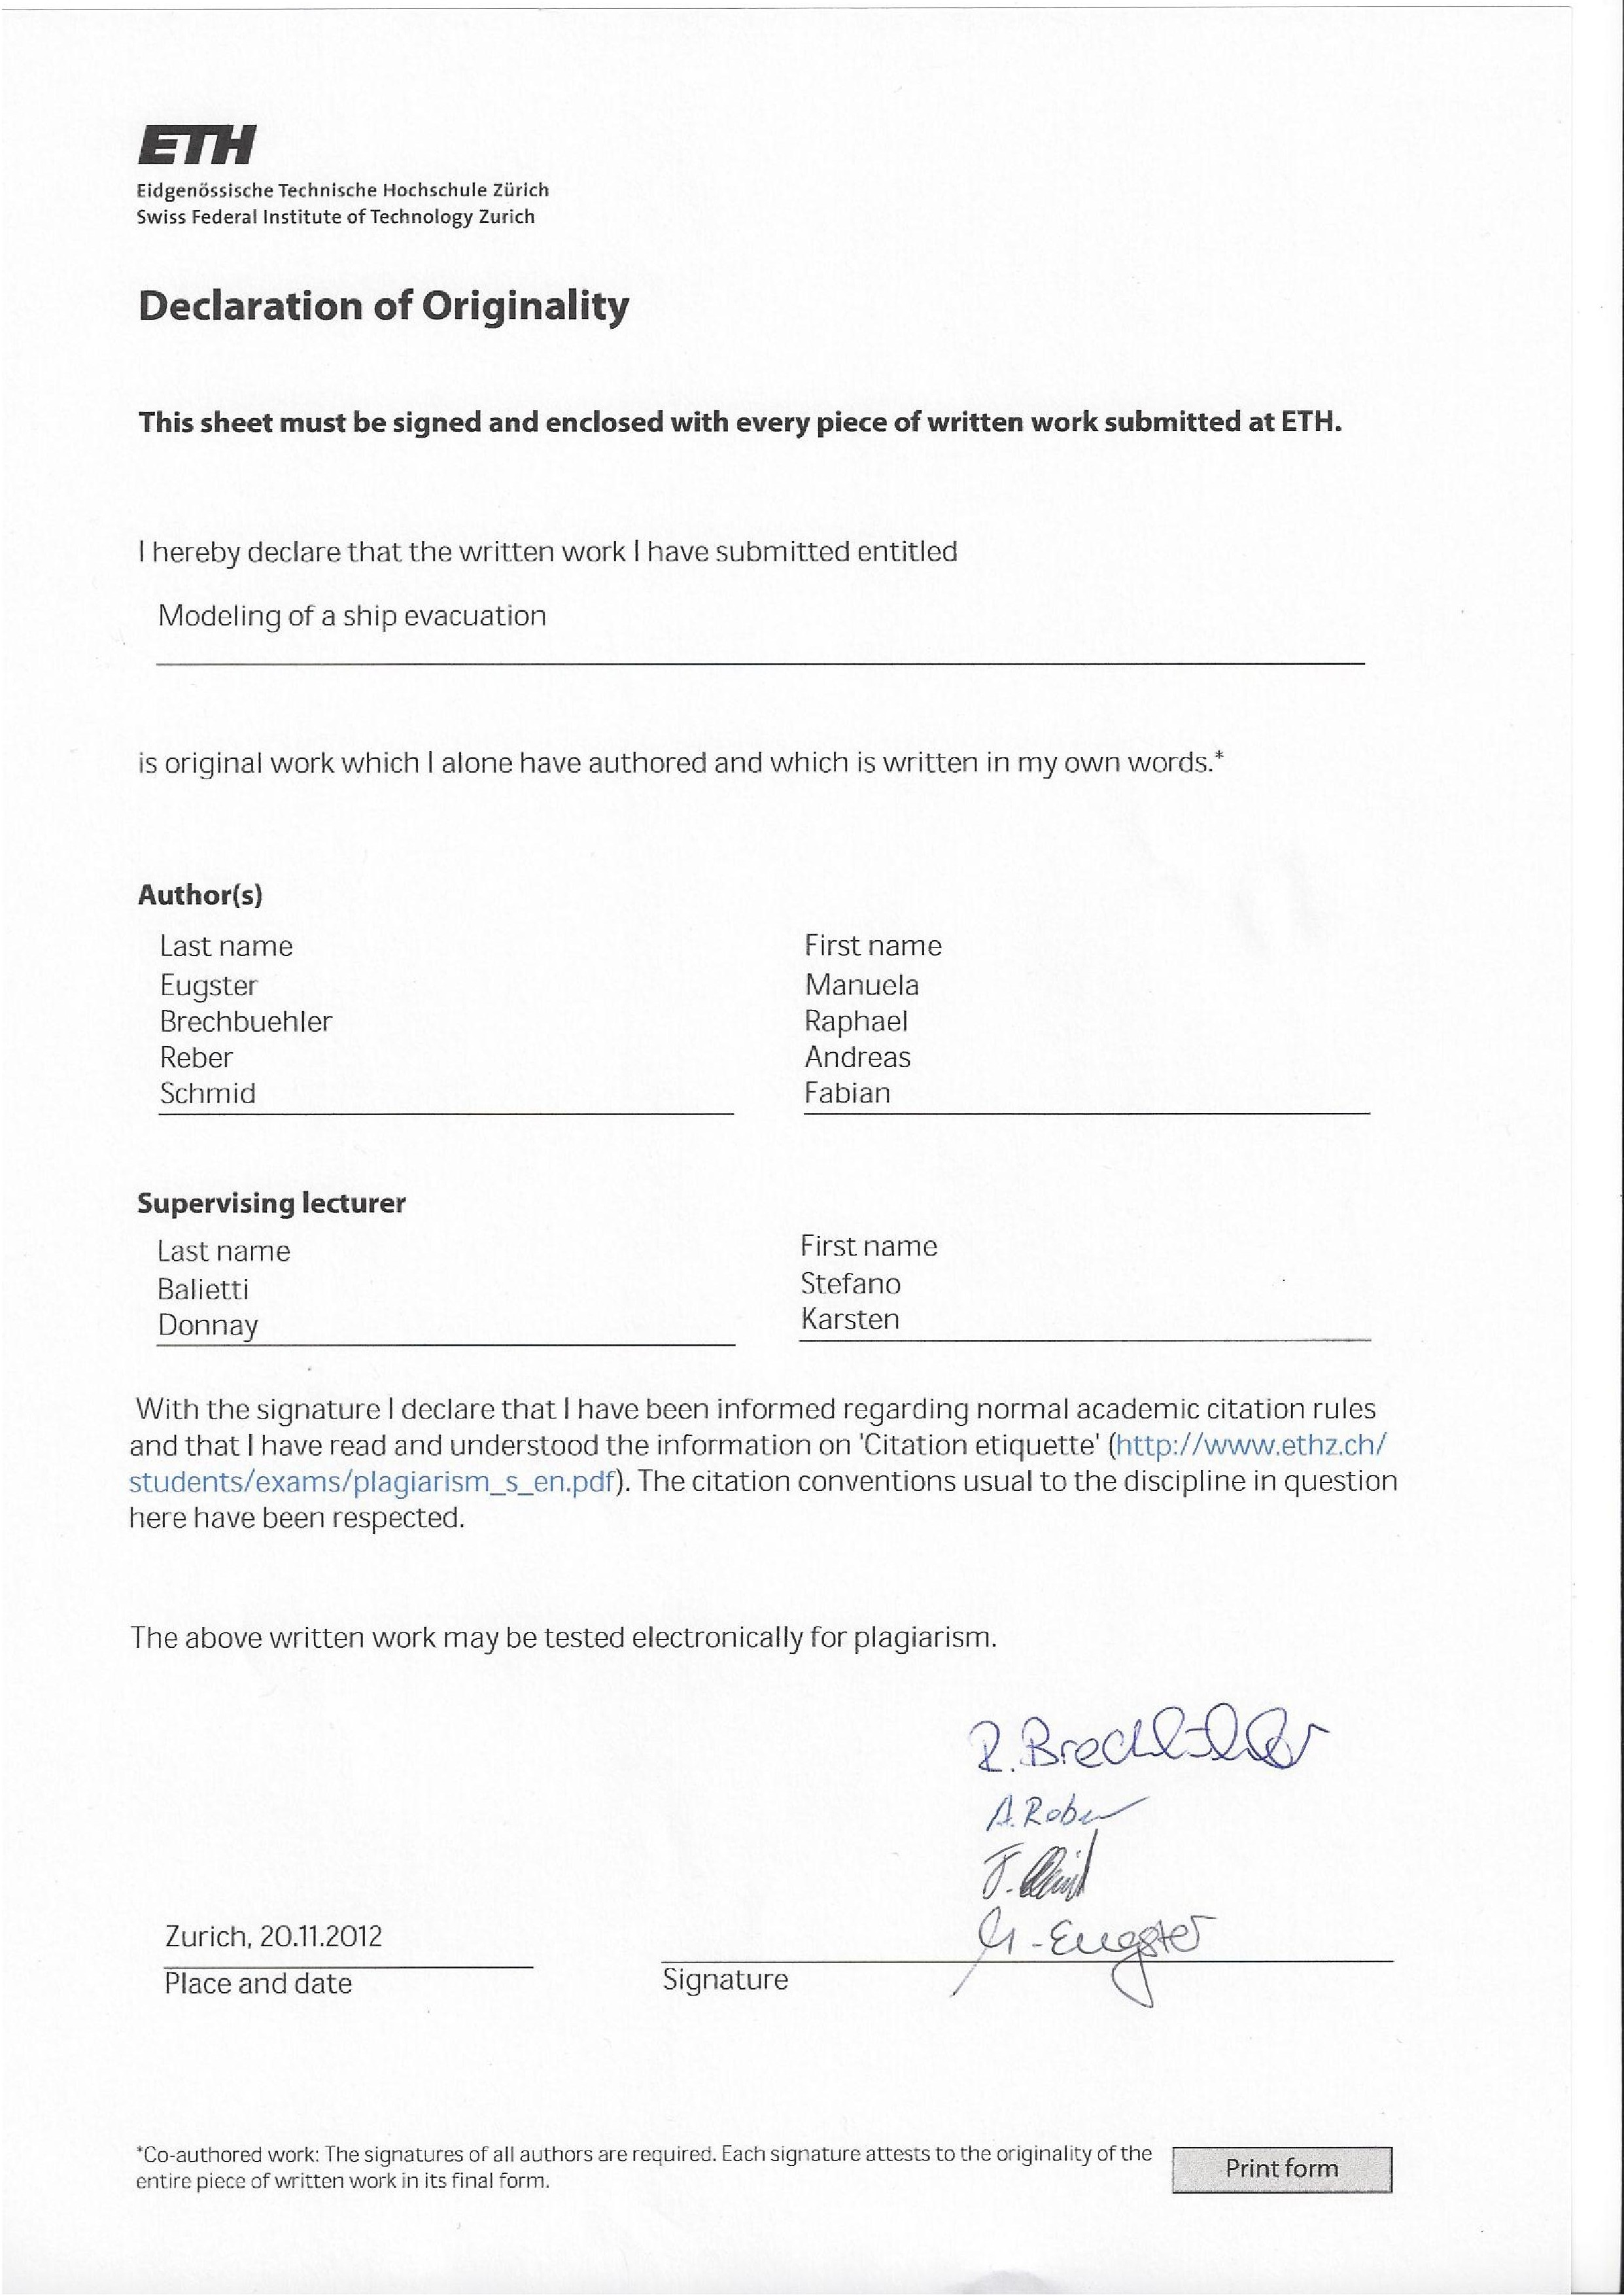
\includegraphics[width=\textwidth]{pics/declaration.jpg}

% IMPORTANT
% you MUST include the ETH declaration of originality here; it is available for download on the course website or at http://www.ethz.ch/faculty/exams/plagiarism/index_EN; it can be printed as pdf and should be filled out in handwriting


%%%%%%%%%% Table of content %%%%%%%%%%%%%%%%%

\tableofcontents

\newpage

%%%%%%%%%%%%%%%%%%%%%%%%%%%%%%%%%%%%%%%



\section{Abstract}
The evacuation of a passenger liner is problematic due to a big mass of passengers wanting to reach the rescue boats. Real data can just be gained on accidents. Another way is to simulate such scenarios using computer models. Our approach was to take a common ship shape with real floor plans and run simulations on it with a continuous space social force model as introduced by Helbling et al \cite{EscapePanic}. A implementation of this has already been done by a former MSSSM group \cite{Building} on building structures. We took this C based code with a MATLAB interface and changed it to our needs. \\\\
Several scenarios were simulated. As a standard we took a simplified floor plan of the passenger liner Costa Serena, a 290 meter long ship with up to more than 4000 passengers. We compared it to modifications in the stair placement as well as rescue boat capacity adjustments. Another idea was to implement the leading and controlling influence of staff on the passengers.\\\\
Our simulations clarified that there is a potential to decrease the overall evacuation time. The most weightily influence had the stair displacement with up to 20\% faster evacuation. on the other hand, the crew influence model seemed to be to simplified. We did not see a lot of improvement in this scenario. However, a more detailed model would probably lead to better results.\\\\
In a future work one could merge our modifications to get an even safer evacuation. The potential exists.




\section{Individual contributions}
The whole project was completed as a team. For sure we took into consideration all the personal backgrounds and  knowledge. That is the reason why Raphael and Manuela focused on implenting the computer code. Whereas Andreas and Fabian concentrated on providing background information, compared the results with the reality and doing its verification. A more detailled breakdown can be seen by looking at the GitHub timeline of our project.





\newpage
\section{Introduction and Motivations}
\subsection{Introduction}
The evacuation of a passenger liner due to fire, sinking or other issues leads to several problems. A large amount of passengers try to safe their lives and get to a rescue boat. Narrow and branched floors, smoke, inflowing water, the absence of illumination, rude passengers and so forth can make the evacuation difficult and reduce the number of survivors.
There are a lot of norms how to minimize the harm of such an evacuation. For example there are rules on the number of rescue boats dependent on the amount of passengers \cite{SOLAS}. With dry runs the staff is prepared for the case of emergency et cetera. In real life ship corridor reproductions, the behavior of distressed people is studied.
Another approach is to model such ship evacuations numerically on the computer. As an example the software maritimeEXODUS by a development team from the University of Greenwich is a computer based evacuation and pedestrian dynamics model that is capable of simulating individual people, behaviour and vessel details. The model includes aspects of people-people, people-structure and people-environment interaction. It is capable of simulating thousands of people in very large ship geometries and can incorporate interaction with fire hazard data such as smoke, heat, toxic gases and angle of heel” \cite{EXODUS}.
Our approach is similarly to model a passenger ship with a common geometrical outline and ground view. In an optimization process we will thereafter look for an ideal ground view, rescue boat distribution and their size to minimize the time needed for evacuation. Finally we will make a statement on possible improvements.
\subsection{Motivation}
Even though modern ocean liners are considered to be safe, the latest occasions attested that there is still potential for evacuation and safety improvements \cite{concordia}. Certainly we know that this science is very advanced and practised since the sinking of the Titanic. Nevertheless knowing that there are still bottlenecks on the ships we are very motivated to detect and eliminate them with our mathematical models.


\subsection{Fundamental Questions}
To find these bottlenecks we run a mathematical model of a ship structure  with several decks and its passengers \cite{shipdecks}. After we localised these places we are interested in the answers of the following questions:\\\\

\newpage
How much time can be saved by varying the dependent variables mentioned below:
\begin{itemize}
\item How much people can be saved by changing the disposition of the specific room types?
\item Where are the bottlenecks during the evacuation? How can they be avoided?\\\\
\end{itemize}
What is the influence of the rescue boats?
\begin{itemize}
\item Are small or bigger boats better?
\item Where do they have to be positioned?
\end{itemize}
We analyse the difference between uncontrolled and controlled passenger flow:
\begin{itemize}
\item Is the crew able to prevent chaos in the evacuation process?
\item What is the best way to lead the passengers out of the ship?
\end{itemize}
In addition we are keen to know if our model is a good abstraction of the reality.

\subsection{Expected Results}
Before making computer simulations we discussed, what we expect as results out of the simulation:
\begin{itemize}
\item Even though modern ships are quite optimized in regard to evacuation time, they are always a compromise between safety and luxury. Therefore we are convinced to find a superior adjustment of the decks geometries to increase the survival rate.
\item Since the rescue boats can not be averaged but are rather concentrated over one or two decks, we consider the staircases as the bottlenecks.
\item In alinging this variables we are persuaded of a reduction of the overall evacuation time.
\item We suppose that smaller and evenly spread rescue boats combined with a higher quantity will scale the evacuation time down. Certainly there is going to be an optimum in size which we are willing to find.
\item By controlling the rescue we assume to detect a huge decrease in evacuation time. Further we have the hypothesis that disorder can be minimized. The crew who is familiar with the decks and the emergency exits is able to guide the passengers in minimum time to the rescue boats.
\item There are many parameters we do not model in our simulation. For example fire and smoke, the tilt of the ship or handicapped and petrified passengers are disregarded. By leaving out this details we get a very simplified model. However, by starting the optimization process by data of a nowadays passenger liner we hope to see some real evacuation dynamics in this system and therefore make conclusion on the fundamental questions.
\end{itemize}

\newpage

\section{Description of the model}
We base our model on the work done by a group of former MSSSM students, by name Hans Hardmeier, Andrin Jenal, Beat Kueng and Felix Thaler \cite{Building}. In their work "Modeling Situations of Evacuation in a Multi-level Building" they wrote a computer program in in the language C with a MATLAB interface to rapidly simulate the evacuation of multi-level buildings.\bigskip

\subsection{Social force model }
Our approach is the social force model described by Helbling, Farkas and Vicsek \cite{EscapePanic}, as summarised below. In order to observe an escape panic situation and especially bottlenecks, they built up a continuous-space model. In mathematical terms they took Newtons second law and introduced a mix of socio psychological and physical forces for each so called pedestrian. 

\begin{equation}
m_{i}\frac{\mathsf{d}\mathbf{v}_{i}}{\mathsf{d}t}=m_{i}f_{D}+\sum \limits_{j(\neq{i})}{f_{ij}}+\sum \limits_{W}{f_{iW}}
\end{equation}

Each pedestrian has his own mass and a direction $e_i^0$ in which he wants to move with a certain velocity $v_i^0$. He tries to adapt his own velocity to the wanted velocity with a given characteristic time $\tau_i$.

\begin{equation}
f_{D}=\frac{v_{i}^{0}(t)\mathbf{e}_{i}^{0}(t)-\mathbf{v}_{i}(t)}{\tau_{i}}
\end{equation}

There are additionally interaction forces $f_{ij}$ between the pedestrian and other people including an exponential part for the tendency of two pedestrians to stay away from each other. The second and third term are zero if the two pedestrians are not in touch. Elsewise there is a force in tangential direction $t$ and in radial direction away from each other. 

\begin{equation}
f_{ij} = \left\{A_{i}exp[(r_{ij}-d_{ij})/B_{i}]+kg(r_{ij}-d_{ij})\right\}\mathbf{n}_{ij}+\kappa g(r_{ij}-d_{ij})\triangle v_{ji}^t\mathbf{t}_{ij}
\end{equation}

To be able to handle with walls there is another forces $f_{iW}$ introduced. Its direction is away from the surrounding walls and the structure is similar to the one for the interaction between pedestrians.

\begin{equation}
f_{iW}=\left\{A_{i}exp[(r_{i}-d_{iW})/B_{i}]+kg(r_{i}-d_{iW})\right\}\mathbf{n}_{iW}-\kappa g(r_{i}-d_{iW})(\mathbf{v}_{i}\cdot\mathbf{t}_{iW})\mathbf{t}_{iW}
\end{equation}
\newpage
\subsection{Ship structure}
To apply the force model on a realistic situation a ship has to be implemented as well. Floor plans from the Costa Serena were taken \cite{shipdecks}. In order to make strong conclusions we want to keep the following variables independent:

\begin{itemize}
\item Number of passengers (4400 agents)
\item Overall capacity of the rescue boats (4680 seats)
\item Ship size (290 meters long) and outer shape \\\\
\end{itemize}

In order to optimize the evacuation time, we change the following dependent variables:
\begin{itemize}
\item Stairs and their positions
\item Rescue boat size, number and position
\item Control of the passenger flow by crew members (e.g. is there staff to lead the passengers and how are they doing it?)
\end{itemize}


\newpage
\section{Implementation}
As mentioned above our code is based on the work of a previous project. Working on a different problem statement we had to make several adjustments and adapt it to our simulation model. In this chapter we will explain the most significant modifications we made. For the exact understanding of the original code and the process of optimization, please refer to the documentation of the previous project group \cite{Building}, especially chapter five and nine or our code in the Appendix.

\subsection{Basic code}
The builders of the code we base on created a flexible model to simulate building structures. The floors can be feed as graphic data into the system where different colors stand for different areas. Black are walls, red stairs up, blue stairs down, green exits and purple agent spawning areas. The data is evaluated in MATLAB in matrices. Information on parameters such as timestep, simulation time, force characteristics et cetera can be read in using a config file which is evaluated on simulation start.\\
With a fast sweeping algorithm in C a vector field is created for every floor pointing in direction of the shortest way towards stairs and exits. In a loop over all passengers the acting forces on them are calculated and via forward Euler converted into velocities. 

\begin{equation}
\mathbf{v}_{i,new} = \mathbf{v}_{i,previous} + \frac{\sum {f}}{m_{i}}dt
\end{equation}

Again with the forward Euler scheme positions are calculated that were reached in a finite timestep.

\begin{equation}
\mathbf{r}_{i,new}=\mathbf{r}_{i,previous}+\mathbf{v}_{i,new}dt
\end{equation}

\subsection{Code adjustments}

This subsection is intended to illustrate the modifications in the code. We explain the difference between our model and the one used in \cite{Building} and the reason why a modification was necessary. Further we define the assumptions we made to minimize the modifications. Finally we specify the modifications and where they take place. 
\\
Those parts are however not essential for the results of our research. They are ment to be an assistance for continuative projects.
\subsubsection{Exits}
\textbf{Reason:}
\newline
The first change which was necessary was due to the fact that the exits in our simulation are not simply on the lowest floor.
\newline
\textbf{Assumption:}
\newline
In case of an emergency all agents are keen to leave the ship as fast as possible. Therefore in our simulation all passengers above the exits floor are only enabled to move down and passengers lower than the exit floor move upstairs.
\newline
\textbf{Function:}
\newline
\textit{applyForcesAndMove.m}
\newline
\textbf{New variables:}
\newline 
To define the floor in which the exits are we introduced a new variable \textit{floor\underline{ }exit} in the config file.
\newline
\textbf{Modifications:}
\newline
Since we defined our exit, we are able to easily modify the code by splitting the loop, in which the force-calculation and the movement of the agents take place, in two parts. First we loop over all floors higher than the exit floor. In those the agents are only allowed to move down. Secondly we do the same for all people in the floors lower than the exit floor where the passengers only can move up. The only floor left is the exit floor where the agents only move towards exits.
\newline
Because of this modification it is not necessary to loop twice over all floors. Consequently our code remains fast and efficient. We also kept the simple concept of vectors out of booleans. This means for each agent there is one number set: 
\begin{itemize}
\item If the agent reaches a staircase and therefore changes the floor 1 is stored in the logical array \textit{floorchange}
\item otherwise a 0 is stored
\end{itemize}
The assumption is also a very helpfull simplification for the pictures since we do not have to mess with the problem of stairs overlapping.


\subsubsection{Different exits}
\textbf{Reason:}
\newline
In our model the exits are the rescueboats, which can only hold a limited number of agents. Therefore we had to find a way how to differ the exits from each other and to assign a specific number to every exit. This number defines how many agents can stay on that rescueboat.
\newline
\textbf{Function:}
\newline
\textit{loadConfig.m}
\newline
\textbf{New variables:}
\newline
- \textit{exit\underline{ }count}, to define the number of exits.\newline
- For each exit \textit{k} a varialbe \textit{exit\underline{ }k\underline{ }nr}, to define the number of agents it can hold.\newline
- To store how many agents can exit in one specific exit, we introduced a matrix \textit{exit\underline{ }nr matrix}, where the number of agents that can exit is indicated for each pixel.
\newline
\textbf{Modifications:}
\newline 
Some changes in the decoding of the pictures were nessecary. The aim was to change as little as possible to the original code. It was clear that we are going to need as many different colors as we have different exits, to be able to distinguish them during the simulation.
\\
We define every pixel which has red to value=0, blue value=0 and green value unequal to zero a "exit-pixel". Now we can specify a lot of different colored exits by using green values between 256 and 256-\textit{exit\underline{ }count}.
\newline
We implemented the matrix \textit{exit\underline{ }nr} similar to the already existing one \textit{img\underline{ }exit}, in which we store a count to number the different exits. The number is defined by the green value of the pixel that belongs to this exit.

\definecolor{commentcolor}{RGB}{89, 168, 89}
\definecolor{keywordcolor}{RGB}{68, 68, 255}
\definecolor{stringcolor}{RGB}{205, 139, 247}
\definecolor{numbercolor}{RGB}{128, 128, 128}
\definecolor{bgcolor}{RGB}{245, 248, 253}

\begin{figure}[h]
\centering
\begin{tabular}
{|>{\large}m{\textwidth}|} \hline
\bigskip

\textcolor{commentcolor}{\%make a zeros matrix as big as img\underline{ }exit}
\newline
config.exit\underline{ }nr=zeros(size(config.floor(config.floor\underline{ }exit).img\underline{ }exit));
\newline
\textcolor{commentcolor}{\% build the exit\underline{ }nr matrix}
\newline
config.exit\underline{ }nr = config.exit\underline{ }nr + e*( img\underline{ }build(:, :, 1) == 0 \& img\underline{ }build(:, :, 2) == (256-e) \& img\underline{ }build(:, :, 3) == 0 ) ;
\bigskip
\\ \hline
\end{tabular}
\caption{Implementation of the exit\underline{ }nr matrix}
\end{figure}
\subsubsection{Closing exits during simulation}

\textbf{Reason:}
\newline
To close an exit as soon as it let a specific number of agents in, we have to keep track of the number of agents that already used this exit.
\newline
\textbf{Function:}
\newline
\textit{loadConfig.m} and \textit{applyForcesAndMove.m}
\newline
 \textbf{New variables:}
\newline
\textit{exit\underline{ }left}
\newline
\textbf{Modifications:}
\newline
For this purpose, we defined the matrix \textit{exit\underline{ }left}, in which we store the number of agents who can exit for every exit.

\begin{figure}[H]
\centering
\begin{tabular}
{|>{\large}m{\textwidth}|} \hline
\bigskip
\textcolor{commentcolor}{\%make a zeros vector as long as exit\underline{ }count}
\newline
config.exit\underline{ }left = zeros(1,config.exit\underline{ }count);
\newline
\textcolor{commentcolor}{\%loop over all exits}
\newline
\textcolor{keywordcolor}{for} e=1:config.exit\underline{ }count
\newline
\textcolor{commentcolor}{\%build the exit\underline{ }nr matrix}
\newline
config.exit\underline{ }nr = config.exit\underline{ }nr + e*( img\underline{ }build(:, :, 1) == 0 \& img\underline{ }build(:, :, 2) == (256-e) \& img\underline{ }build(:, :, 3) == 0 ) ;
\newline
\textcolor{commentcolor}{\%build the exit\underline{ }left matrix and save the number of agents the exit can hold}
\newline
config.exit\underline{ }left(1,e) = config.(sprintf(\textcolor{stringcolor}{'exit\underline{ }\%d\underline{ }nr'}, e)); 
\newline
\textcolor{keywordcolor}{end}
\bigskip
\\ \hline
\end{tabular}
\caption{Implementation of the exit\underline{ }left matrix}
\end{figure}
\bigskip
In the loop where the forces and velocities are updated, (\textit{applyForcesandMove.m}) we added a piece of code, which updates the exit\underline{ }left matrix at every timestep.
\newline
First, we get the number of the current exit.
\begin{figure}[h!]
\centering
\begin{tabular}
{|>{\large}m{\textwidth}|} \hline
\bigskip
\textcolor{commentcolor}{\%save current exit nr}
\newline
data.current\underline{ }exit = data.exit\underline{ }nr(round(newp(1)), round(newp(2)));
\bigskip
\\ \hline
\end{tabular}
\caption{Implementation to get the current exit number}
\end{figure}
\\
Then we update the \textit{exit\underline{ }left} matrix by counting down the number of agents allowed to exit by 1. 
\begin{figure}[h!]
\centering
\begin{tabular}
{|>{\large}m{\textwidth}|} \hline
\bigskip
\textcolor{commentcolor}{\%update exit\underline{ }left}
\newline
data.exit\underline{ }left(1,data.current\underline{ }exit) = data.exit\underline{ }left(1,data.exit\underline{ }nr(round(newp(1)), round(newp(2)))) - 1;
\bigskip
\\ \hline
\end{tabular}
\caption{Implementation to update the exit\underline{ }left}
\end{figure}
If the allowed number of agents exited the number is 0. Now we have to close the current exit, by changing it into a wall. Therefore we have to update the \textit{img\underline{ }wall} matrix.
\begin{figure}[h!]
\centering
\begin{tabular}
{|>{\large}m{\textwidth}|} \hline
\bigskip
\textcolor{commentcolor}{\%close exit if there is no more free space}
\newline
\textcolor{keywordcolor}{if} data.exit\underline{ } left(1,data.current\underline{ }exit) $<$ 1
\newline
\textcolor{commentcolor}{\%change current exit to wall}
\newline
data.floor(data.floor\underline{ }exit).img\underline{ }wall = data.floor(data.floor\underline{ }exit).img\underline{ }wall == 1 \textcolor{blue}{...}
\newline
| (data.exit\underline{ }nr == (data.current\underline{ }exit));
\newline
data.floor(data.floor\underline{ }exit).img\underline{ }exit = data.floor(data.floor\underline{ }exit).img\underline{ }exit == 1 \textcolor{blue}{...}
\newline
\& (data.exit\underline{ }nr ~= (data.current\underline{ }exit));
\bigskip
\\ \hline
\end{tabular}
\caption{Implementation to close filled  boats}
\end{figure}


\subsection{Crew command simulation}
\textbf{Reason:}
\newline 
In reality an evacuation is coordinated. Loudspeaker announcements and crew members lead the people to the exit floor. In some cases there are even assembly points on the deck where people meet. Afterwards they go with crew members to the rescue boats.
In our first simulations we saw, that the last passengers escaping the ship have to walk all the way along the ship to get into a rescue boat in the middle of the deck. Those boats are the only ones that are not fully loaded at this time. To counteract, we tried to implement somehow the interaction of the passengers and the crew members. 
\newline
\textbf{Assumption:}
\newline 
In order not to change to much the structure of our standard evacuation code, we tried to implement the scenario in two steps. First just some rescue boats in the middle of the ship are available what can be interpreted as a crew leading people to those boats because they know that the boats near to the stairs should be left unalloyed for the last passengers to be evacuated rapidly. In a second step, all rescue boats are opened when a certain number of passengers already left the ship.
 \newline
\textbf{Function:}
\newline 
The whole basic code has been copied and ajusted in several positions, mainly in loadConfig.m and applyForcesAndMove.m.



\subsection{Video creation}
\textbf{Reason:}
\newline
In the basic code there was a graphical output into eps-formated files possible on every timestep. The images then had to be converted into a video file in a postprocessing part. This is not an optimal implementation for a fast system. Furthermore it turned out that we could increase the simulation speed by factor two just by saving not on every single timestep but only on every 10$^t$$^h$ or 100$^t$$^h$. Another issue was the conversion from eps to a video file. To simplify the handling, we used a MATLAB function to create directly a video out of the figures instead of making a detour via images.
\newline
\textbf{Function:}
\newline
\textit{simulate.m, initialize.m}
\newline
\textbf{New variables:}
\newline
\textit{save\underline{ }frame}
\newline
%\textbf{Modification:}
%\newline
%
%\begin{figure}[H]
%\centering
%\begin{tabular}
%{|>{\large}m{\textwidth}|} \hline
%\bigskip
%\textcolor{commentcolor}{\% prepare video file name}
%\newline
%data.video\underline{ }file\underline{ }name = [\textcolor{stringcolor}{$'$video\underline{ }$'$} data.frame\underline{ }basename \textcolor{magenta}{$'$.avi$'$}];
%\newline
%\newline
%\textcolor{commentcolor}{\% make video while simulation}
%\newline
%\textcolor{keywordcolor}{If} data.save\underline{ }frames==1
%\newline
%             vidObj=VideoWriter(data.video\underline{ }file\underline{ }name);
%\newline
%             open(vidObj);
%\newline
%\textcolor{keywordcolor}{end}
%\newline
%\newline
%\textcolor{commentcolor}{\% make video while simulate   }
%\newline
%currFrame=getframe(data.figure\underline{ }floors);
%\newline
%writeVideo(vidObj,currFrame);
%\newline
%\newline
%\textcolor{commentcolor}{\% make video while simulation}
%\newline
%currFrame=getframe(data.figure\underline{ }floors);
%\newline
%writeVideo(vidObj,currFrame);
%\newline
%\newline
%\textcolor{commentcolor}{\% make video while simulation}
%\newline
%close(vidObj);
%\bigskip
%\\ \hline
%\end{tabular}
%\caption{Implementation to produce video file}
%\end{figure}

\subsection{System output}
\textbf{Reason:}
\newline
Storing the simulation output is important to be able to analyse and optimize the system. The output of the basic code was just a plot with agents left the building over time and the above mentioned graphical output of the floor plans over time. We extended the output and created a dump struct where all the important variables are listed over time. That struct is the system output at simulation end and it can be used in a postprocessing part to generate meaningful graphs and data.
\newline
\textbf{Function:}
\newline
\textit{simulate.m}
\newline
\textbf{New variables:}
\newline
\textit{output}
\newline
%\newpage
%\textbf{Modification:}
%
%\begin{figure}[H]
%\centering
%\begin{tabular}
%{|>{\large}m{\textwidth}|} \hline
%\bigskip
%\textcolor{commentcolor}{\% init output matrizes}
%\newline
%data.output = struct;
%\newline
%data.output.config = config;
%\newline
%data.output.agents\underline{ }per\underline{ }floor = ones(data.floor\underline{ }count,data.duration/data.dt).$*$(-1);
%\newline
%data.output.exit\underline{ }left = zeros(data.exit\underline{ }count,data.duration/data.dt);
%\newline
%\newline
%\textcolor{commentcolor}{\% prepare output file name}
%\newline
%data.output\underline{ }file\underline{ }name = [\textcolor{magenta}{$'$output\underline{ }$'$} data.frame\underline{ }basename];
%\newline
%\newline
%\textcolor{commentcolor}{\% set deleted\underline{ }agents to zero}
%\newline
%data.output.deleted\underline{ }agents = 0;
%\newline
%\newline
%\textcolor{commentcolor}{\% dump agents\underline{ }per\underline{ }floor to output }
%\newline
%\textcolor{keywordcolor}{for} floor=1:data.floor\underline{ }count
%\newline
%data.output.agents\underline{ }per\underline{ }floor(floor,data.step) = length(data.floor(floor).agents);
%\newline
%\textcolor{keywordcolor}{end}
%\newline
%\newline
%\textcolor{commentcolor}{\% dump exit\underline{ }left to output}
%\newline
%data.output.exit\underline{ }left(:,data.step) = data.exit\underline{ }left';
%\newline
%\newline
%\textcolor{commentcolor}{\% toc of whole simulation}
%\newline
%data.output.simulation\underline{ }time = toc(simstart);
%\newline
%\newline
%\textcolor{commentcolor}{\% save output}
%\newline
%output = data.output;
%\newline
%save(data.output\underline{ }file\underline{ }name,\textcolor{stringcolor}{$'$output$'$})
%\newline
%fprintf('\textcolor{stringcolor}{$'$Frame \%i done (took \%.3fs; \%.3fs out of \%.3gs simulated). n$'$}, 
%\newline
%data.step, data.telapsed, data.time, data.duration);
%\newline
%\newline
%\textcolor{commentcolor}{\% save complete simulation}
%\newline
%output = data.output;
%\newline
%save(textcolor{stringcolor}{$'$output$'$,$'$output$'$})
%\bigskip
%\\ \hline
%\end{tabular}
%\caption{Implementation to produce the output}
%\end{figure}

\subsection{Postprocessing}
\textbf{Reason:}
\newline
To analyse the gathered data in a systematic way and to create consistent plots we created a postprocessing file. The output file can be loaded in MATLAB using the load command and is thereafter automatically evaluated. Plots with agents per floor over time, left space in rescue boats over time and agents that left the ship over time are created with proper axis label and so on. Additionally there is an output in the MATLAB command window with timestep, number of steps, total simulation time, agents on ship on start, agents on ship on simulation end, agents deleted due to Not-a-Number-positions and the characteristic $t_{10}$, $t_{50}$, $t_{90}$ and $t_{95}$ times.
\newline
\textbf{Function:}
\newline
\textit{postprocessing.m}
\newline
\textbf{New variables:}
\newline
none of relevance
\newline
\textbf{Modification:}
\newline
We created the whole script ourself. It can be found in the annex.
\subsection{Parameter input and config file}
The social force model can be adjusted using different parameters e.g. to weight the importance of different forces among each other or to define the decay rate of these forces over the distance. Also the mass and radii of the passengers as well as their maximum velocity can be set. The parameters are written down in the config files that are passed to the MATLAB interface on simulation start. For sake of simplicity we adopted the force model parameters from the previous group. The parameters concerning the ship shape were adjusted so that they represent reality as far as possible.
\newline
In the annex a typical simulation input of the config file and some explanations can be found.

\subsection{Ship Decks}

The Costa Concordia has 14 decks which are all different from each other. They are connected by stairs and elevators in different configurations and they fulfilll different purposes. There are decks for entertainment, eating, shopping, sports and so on.
Due to the big differences of each deck, it is enormous time consuming to implement all these decks with all details in a model. So it is necessary to simplify the decks in a reasonable manner.
Further the picture source is not perfect in size and data type so there is a manual conversion needed.
In this chapter it is shown what assumptions were made and with which conversion techniques the decks were implemented into the model.

\subsubsection{Conversion}
First of all the decks have to match each other in pixel size and position to allow a flawless connection of the decks. So the size of some decks has to be adjusted and the stair overlay has to be matched as good as possible.
Secondly doors, numbers, names and symbols are removed to have one connected surface without unreal obstacles.
\newline
Now that the surfaces are clean and connected, the colours have to be replaced by predefined colours of the code (purple for spawn of agents, black for walls, red for upstairs, blue for downstairs and different green type for each rescue boat).
\newline
In figures \ref{Deck-stairs} and \ref{Deck-elevator} a small portion of a deck with stairs, rooms, doors and elevators is shown before and after conversion. In the converted picture is a blue block included for the stairs, which conversion will just be explained in the next part.

\begin{figure}[H]
\centering
{\begin{minipage}[t]{7.4cm}
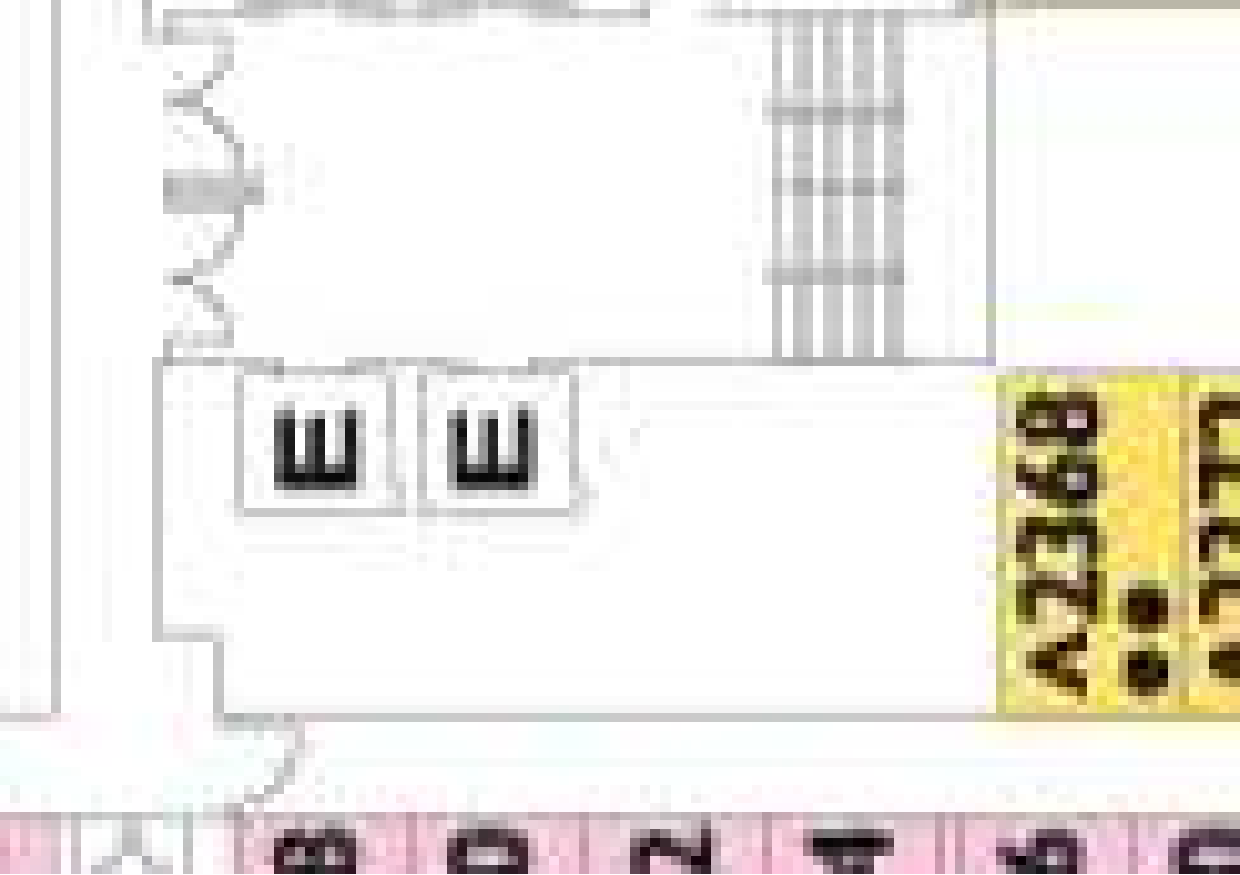
\includegraphics[width=\textwidth]{pics/Decksetup-stairs.pdf}
\caption{Deck before conversion}
\label{Deck-stairs}
\end{minipage}}
{\begin{minipage}[t]{7.4cm}
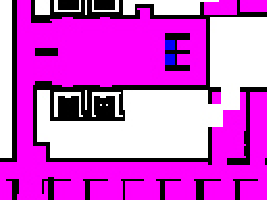
\includegraphics[width=\textwidth]{pics/deckconversion2.pdf}
\caption{Deck after conversion}
\label{Deck-elevator}
\end{minipage}}
\end{figure}

In most of the cases stairs from one to another floor are designed in a spiral way to minimize the consumed space. That leads to a problem by implementing the stairs into the model. It is not possible to make a clean transition from one floor to another without using some tricks.
\newline
There are special additional floors to overcome the mentioned problem in the work "Modeling Situations of Evacuation in a Multi-level Building"\cite{Building}. These additional floors which represents the stairs, are a fine method to create an infinite amount of floors and connections without any trouble. But it needs an additional floor for each connection.
\newline
While the agents on the ship march only in the direction of the rescue floor the connection can be simplified. So there is a new technique used to get rid of these additional floors.
\newline
In figure \ref{Decktwostairs} a spiralling stairs connection between floor 01 and floor 02 is shown as example. The arrows in light blue are used to clarify the technique.
\newline
The agents arrive from the left on floor 11 and go into the direction of the arrow until they reach the blue box. There they are skipped down on  the floor 10 and try to go to the blue box again. So they have to go around to be skipped down again on floor 09 and go around in the other direction. That continues until they reach floor 04 which is the floor with the rescue boats.

With that technique no additional floors are needed and we get very close to the real spiralling stairs. For the ship in that project this is sufficient, because the modelling fault will be in a lower degree than the one of other assumptions.

\begin{figure}[H]
\centering
{\begin{minipage}[t]{7.4cm}
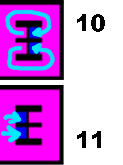
\includegraphics [width=0.5\textwidth]{pics/Decktwostairs.pdf}
\caption{Stairs connection between floor 10 and floor 11}
\label{Decktwostairs}
\end{minipage}}
\end{figure}

\subsubsection{Similarities and reduction}
The most important floor for the simulation is of course floor 04 because it holds all the rescue boats as seen in figure \ref{Decksconverted}. There all agents have to pass and it is reasonable to have it very detailed. Floor 05 and 03 are the ones just above and beyond and will also have a non neglectable influence on the agent’s movement.
\newline
The further we move the less important the deck configuration gets, because it is assumed that the stairs will be the bottlenecks. As long as the stair setup corresponds good to reality, the further decks can differ more.
So we decided to convert deck 02, 03, 04 and 05 in detail and make a copy with adjusted stairs for each other floor. Floor 02 is used for the copy because it gets the closest to floor 01, 06 and 07 and is by that still a good approximation.
\newline
Floor 08 until 14 differ more from floor 02 but as long as they are far away from floor 04 it will not have a big influence. These last floors are also smaller than floor 02 and therefore the amount of floors is reduced to only 11 with approximately the same area as the original 14 floors.

\begin{figure}[H]
\centering
{\begin{minipage}[t]{7.4cm}
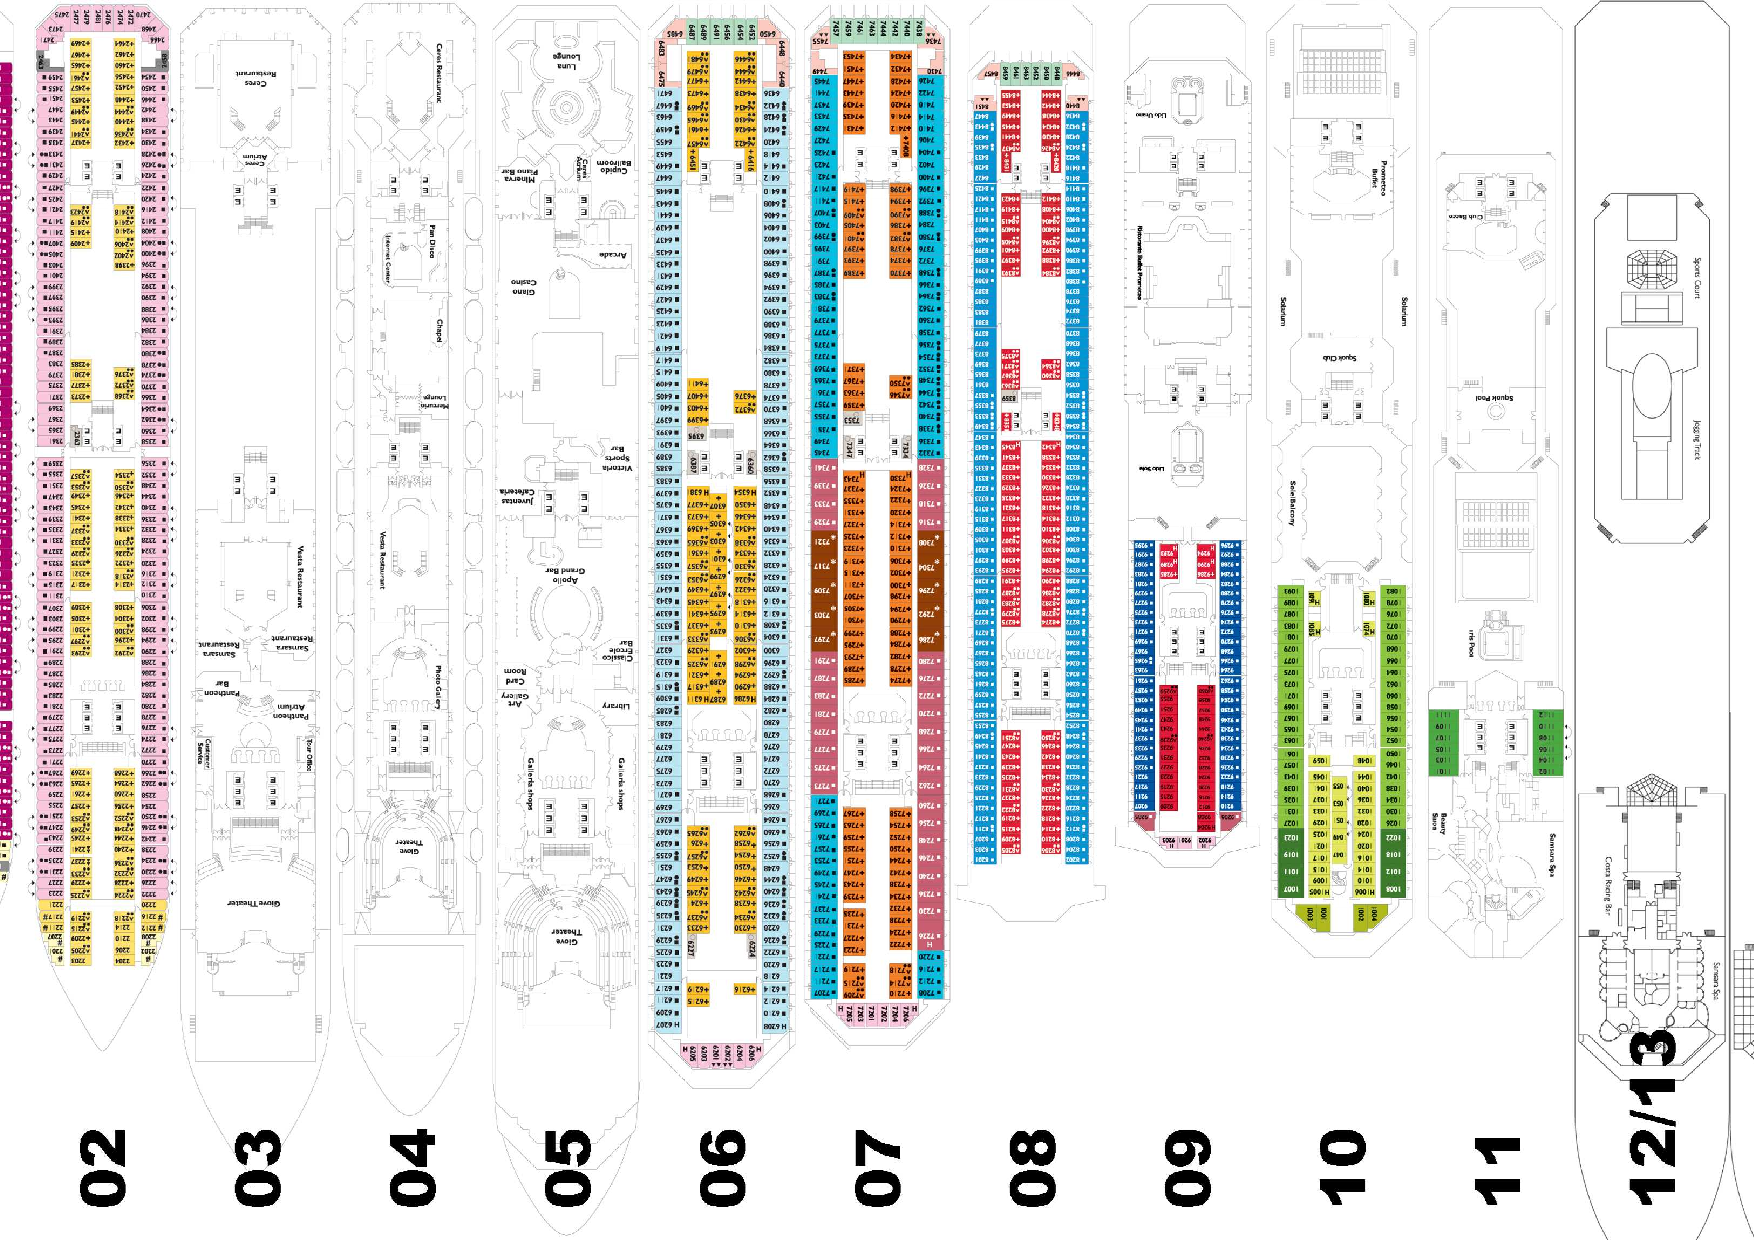
\includegraphics[angle=-90,width=\textwidth]{pics/Decks.pdf}
\caption{Originaldecks before conversion}
\label{Decks}
\end{minipage}}
{\begin{minipage}[t]{7.4cm}
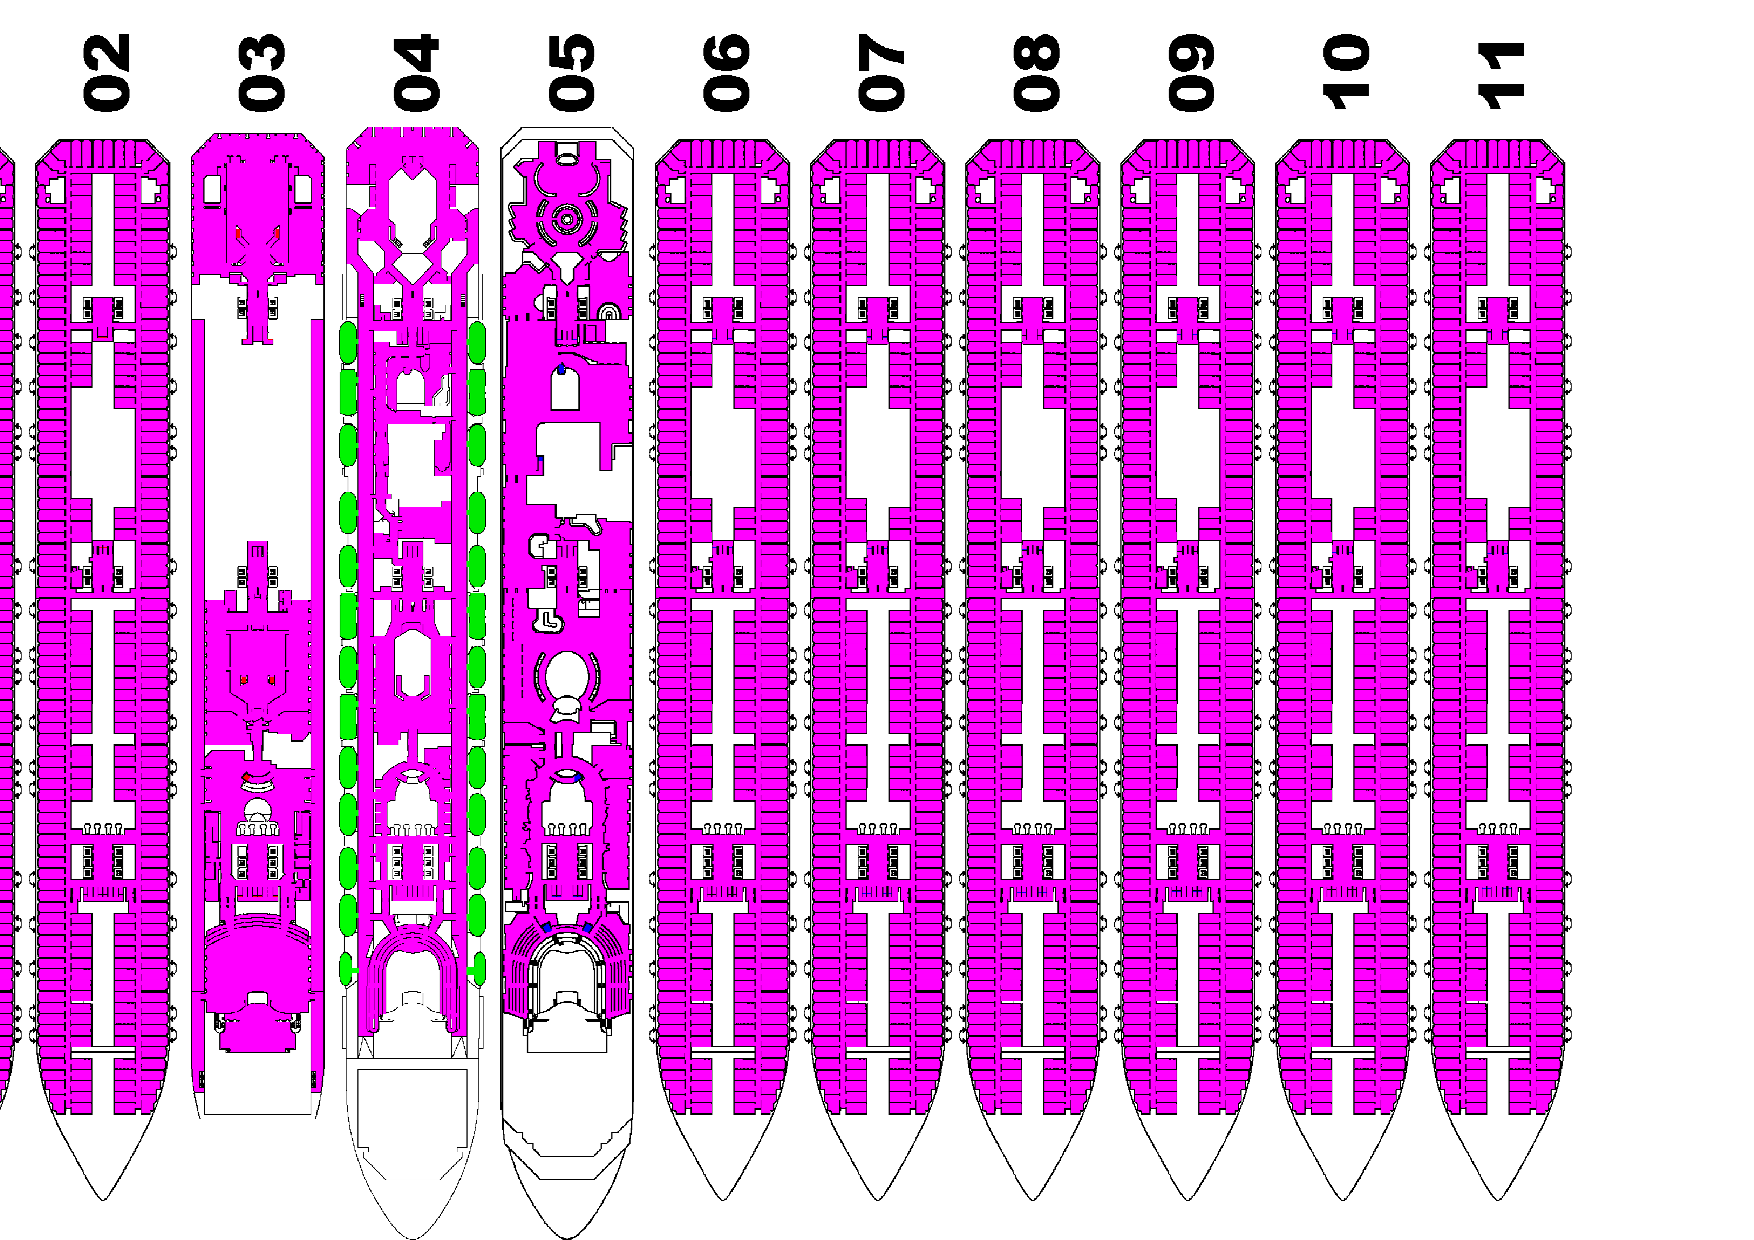
\includegraphics[angle=-90,width=\textwidth]{pics/Decksconverted.pdf}
\caption{Deck approximated and converted}
\label{Decksconverted}
\end{minipage}}
\end{figure}






\newpage
\section{Results and Discussion}

\subsection{Simulation issues}
Some agents always stuck in the walls near the stairways. Those agents did not reach the exits. This is why we could not get a $t_{100}$ time but just saved about 98\% of all passengers. The frequency of this issue was especially high in small areas and with a high total passenger amount. However, there was a trade off between realistic clogging in stairways and good ratio of rescued people out of all passengers. We decided not to decrease the number of passengers or expand the stairs because we did not want to eliminate the realistic clogging behaviour which is important for the simulation.

\subsection{Simulation Results}
\subsubsection{Standard ship}
As listed above we were interested in the time in which a certain percentage of all agents was evacuated:
\newline

\begin{table}[H]
\centering
\begin{tabular}
{|>{\large}m{2cm} |>{\center}b{1.1cm} |>{\center}b{1.1cm}|>{}b{1.1cm}|>{}b{1.1cm}|} \hline \hline
percentage of agents& 10\% &  50\% & 90\% &95\% \\ \hline
evacuation time run1 & 16s &69s & 167s & 214s \\ \hline 
evacuation time run2 & 16s &69s & 164s & 238s \\ \hline 
averaged evacuation time & 16s &69s &166s &226s \\ \hline \hline

\end{tabular}
\caption{Standard simulation: Needed time to evacuate a certain percentage of all agents.}
\end{table}

Further our standard ship simulation showed the following performance:

\begin{figure}[htbp]
\centering
{\begin{minipage}[t]{7.4cm}
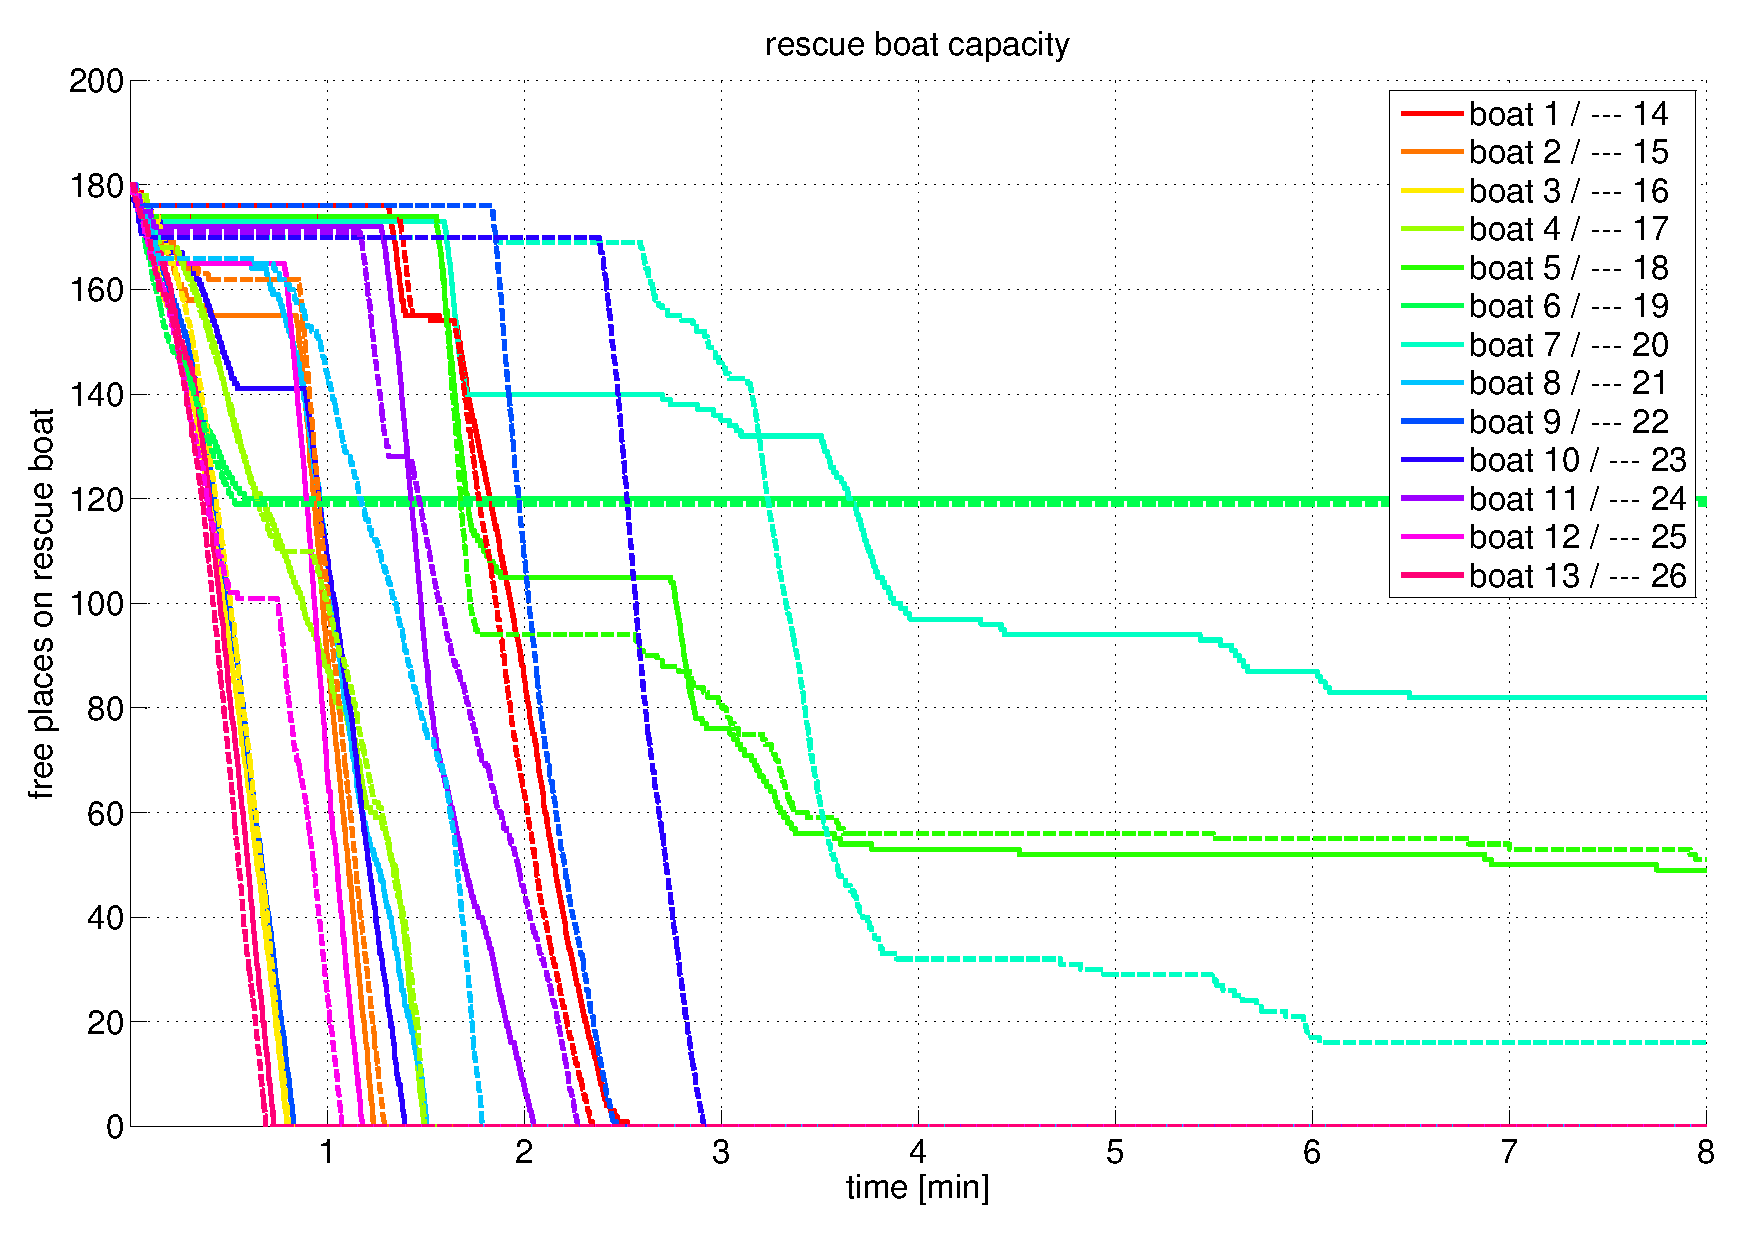
\includegraphics[width=\textwidth]{pics/standard_cap1.pdf}
\caption{Standard simulation: Boat capacities during first simulation}
\end{minipage}}
{\begin{minipage}[t]{7.4cm}
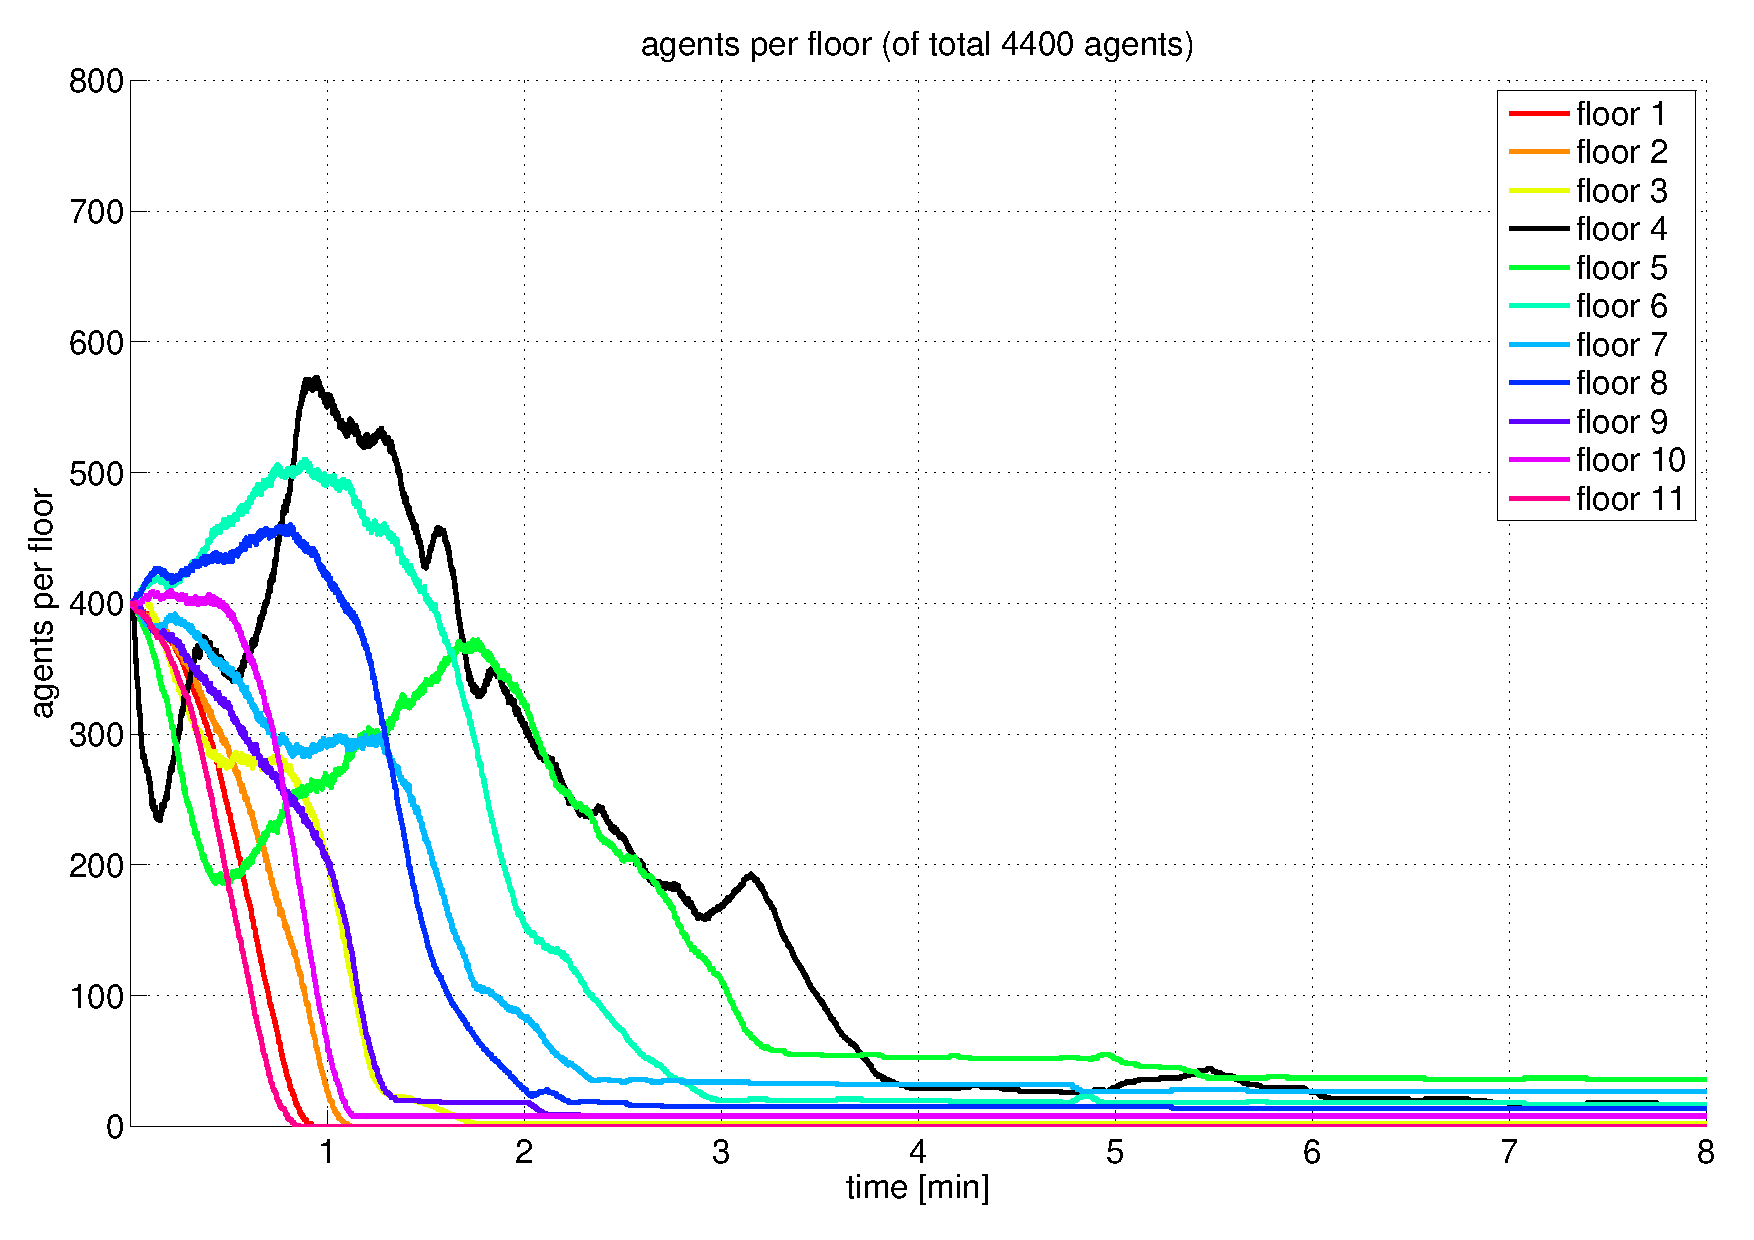
\includegraphics[width=\textwidth]{pics/standard_agents1.pdf}
\caption{Standard simulation: Number of agents per floor in first simulation}
\end{minipage}}
\end{figure}

\subsubsection{Modified room disposition}
As we expected the standard simulation revealed that hold-up problems occur because of the staircases. As the flow everywhere else was quite dynamic we abstained from adjusting the room disposition but instead we inserted an additional staircase. This simulation yielded the following results:

\begin{table}[H]
\centering
\begin{tabular}
{|>{\large}m{2cm} |>{\center}b{1.1cm} |>{\center}b{1.1cm}|>{}b{1.1cm}|>{}b{1.1cm}|} \hline \hline
percentage of agents & 10\% &  50\% & 90\% & 95\% \\ \hline
evacuation time & 16s &67s & 145s & 182s \\ \hline \hline
\end{tabular}
\caption{Added stairs simulation: Needed time to evacuate a certain percentage of all agents.}
\end{table}

\begin{figure}[H]
\centering
{\begin{minipage}[t]{7.4cm}
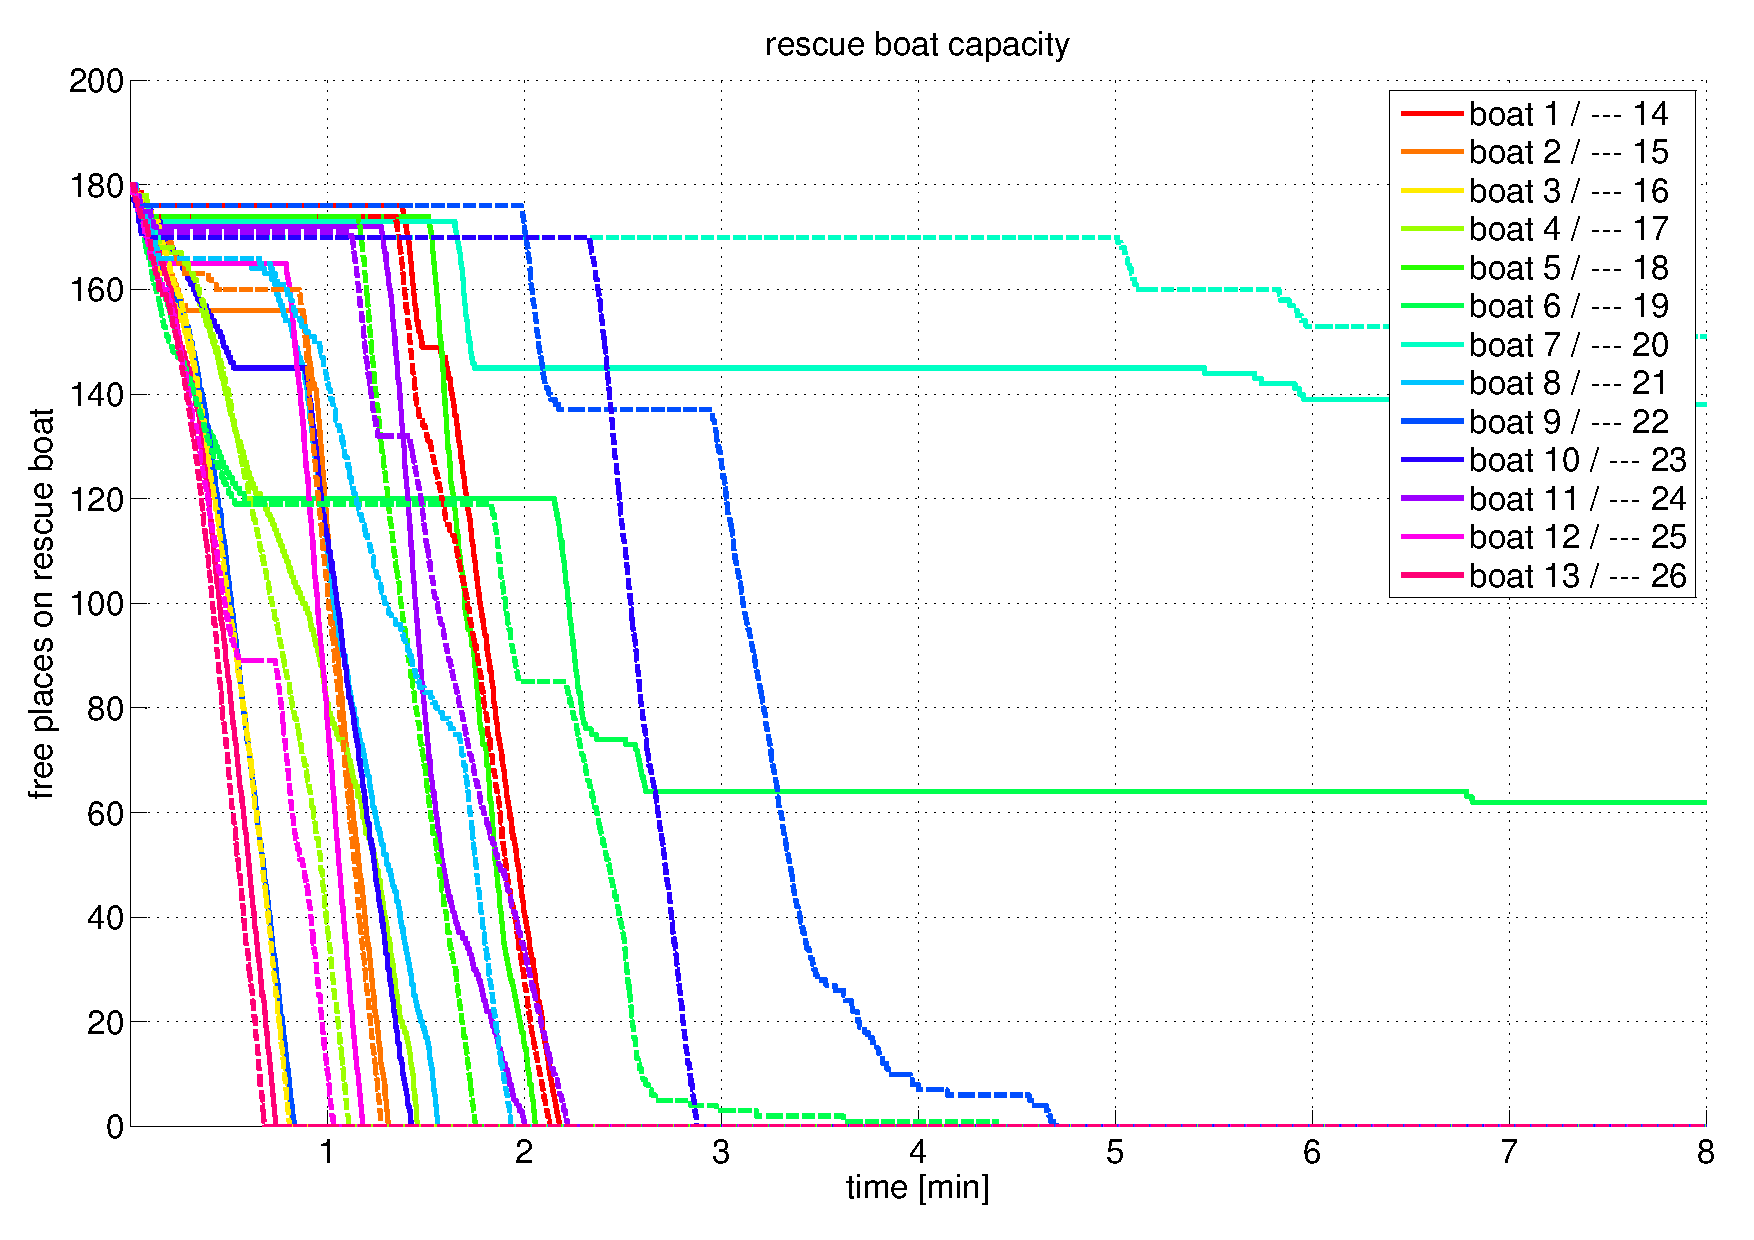
\includegraphics[width=\textwidth]{pics/added_stairs_cap.pdf}
\caption{Added stairs simulation: Boat capacities during simulation}
\end{minipage}}
{\begin{minipage}[t]{7.4cm}
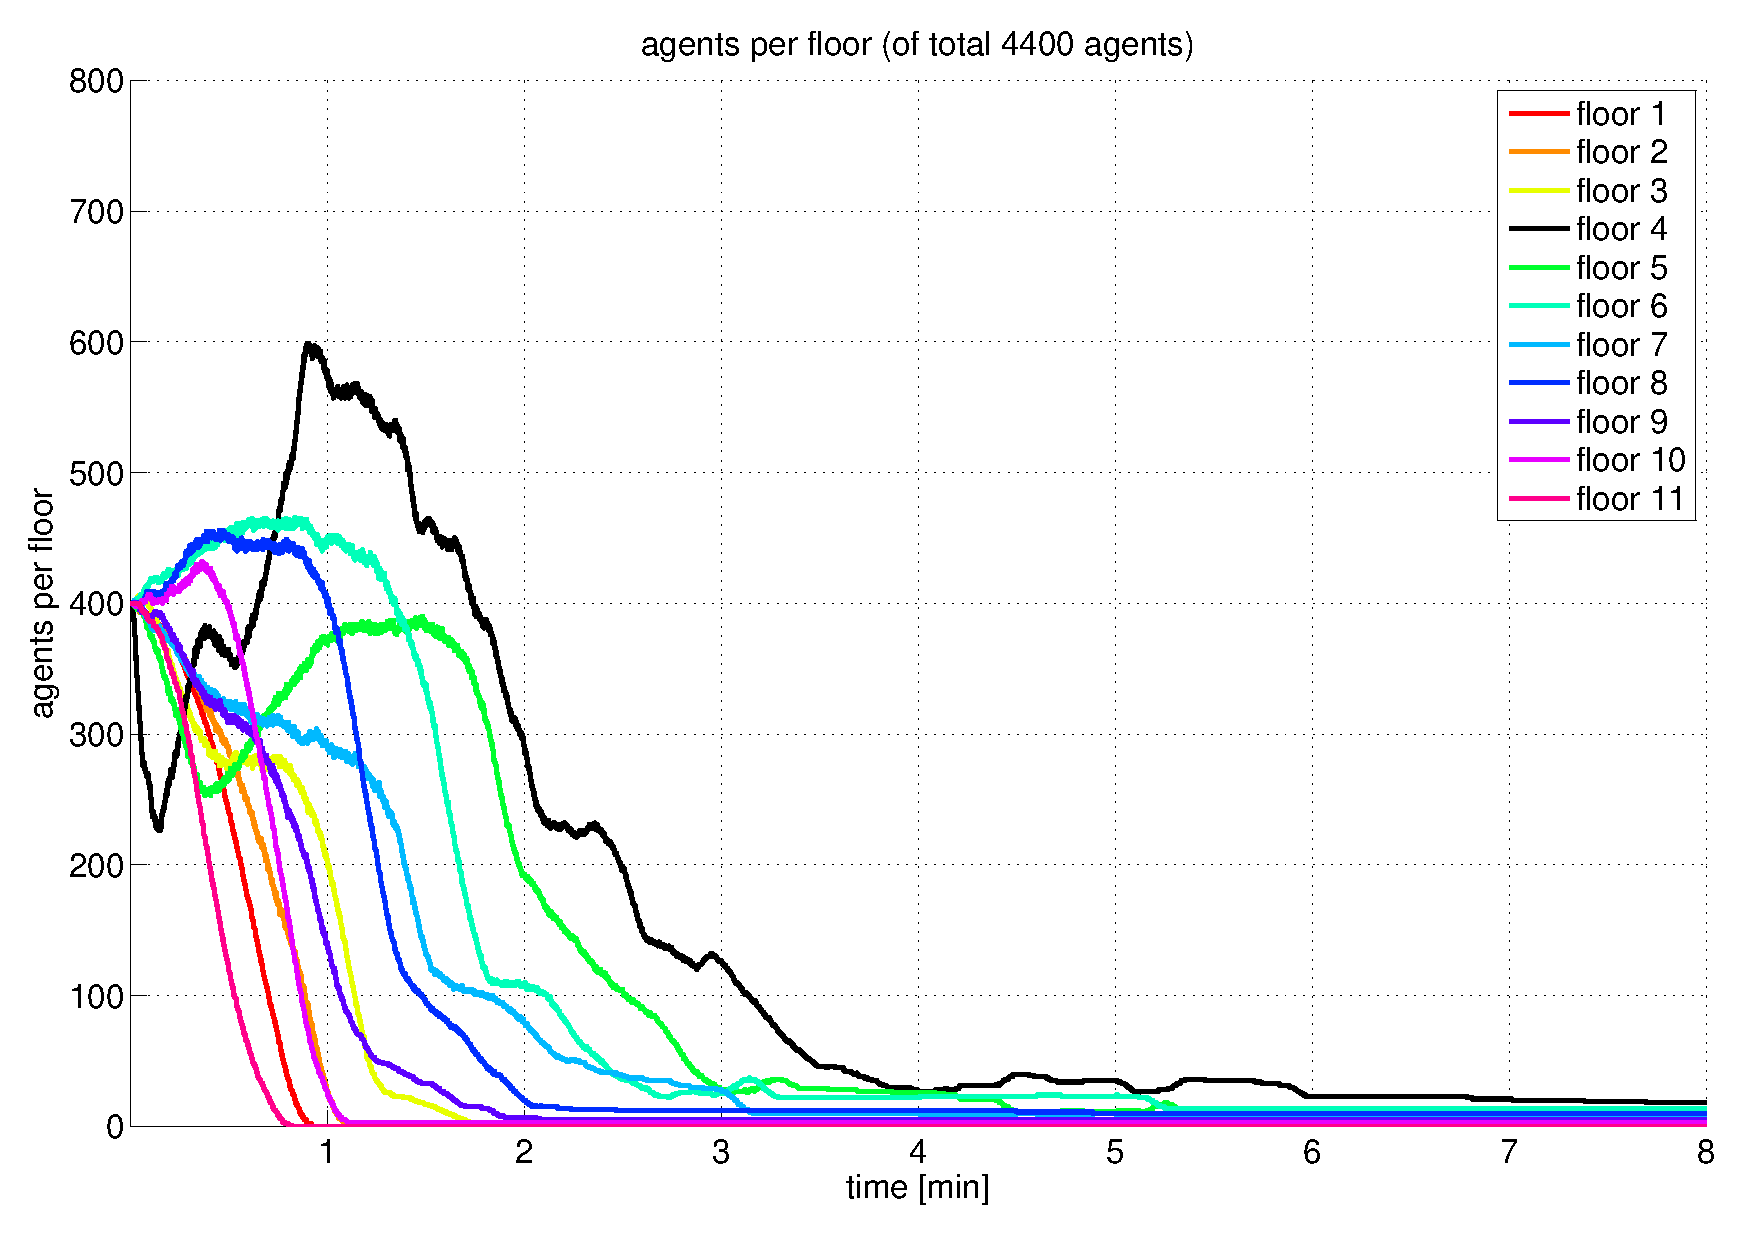
\includegraphics[width=\textwidth]{pics/added_stairs_agents.pdf}
\caption{Added stairs simulation: Number of agents per floor}
\end{minipage}}
\end{figure}
 
\subsubsection{Modified rescueboat size}
As we could see in the simulations with the standard ship, the rescueboats which are nearest to the stairs are filled first. This behavior is very intuitive. As soon as the nearest lifeboats are full, the agents continue to fill the other lifeboats. 
The greatest extension of the evacuation time occurs as follows:
Towards the end of the simulation, not all lifeboats are still open. Therefore leftover agents, which walked in the direction of a lifeboat that closed in the meantime, have to cross a big distance to reach a lifeboat with free space.\newline
We tried to avoid this delay by increasing the capacity of lifeboats near the stairs and removed some, which are the farthest away for the agents left over towards the end of the evacuation.


\begin{table}[H]
\centering
\begin{tabular}
{|>{\large}m{2cm} |>{\center}b{1.1cm} |>{\center}b{1.1cm}|>{}b{1.1cm}|>{}b{1.1cm}|} \hline \hline
percentage of agents & 10\% &  50\% & 90\% & 95\% \\ \hline
evacuation time & 17s &70s & 154s & 203s \\ \hline \hline
\end{tabular}
\caption{Varied boatsize simulation: Needed time to evacuate a certain percentage of all agents.}
\end{table}


\begin{figure}[H]
\centering
{\begin{minipage}[t]{7.4cm}
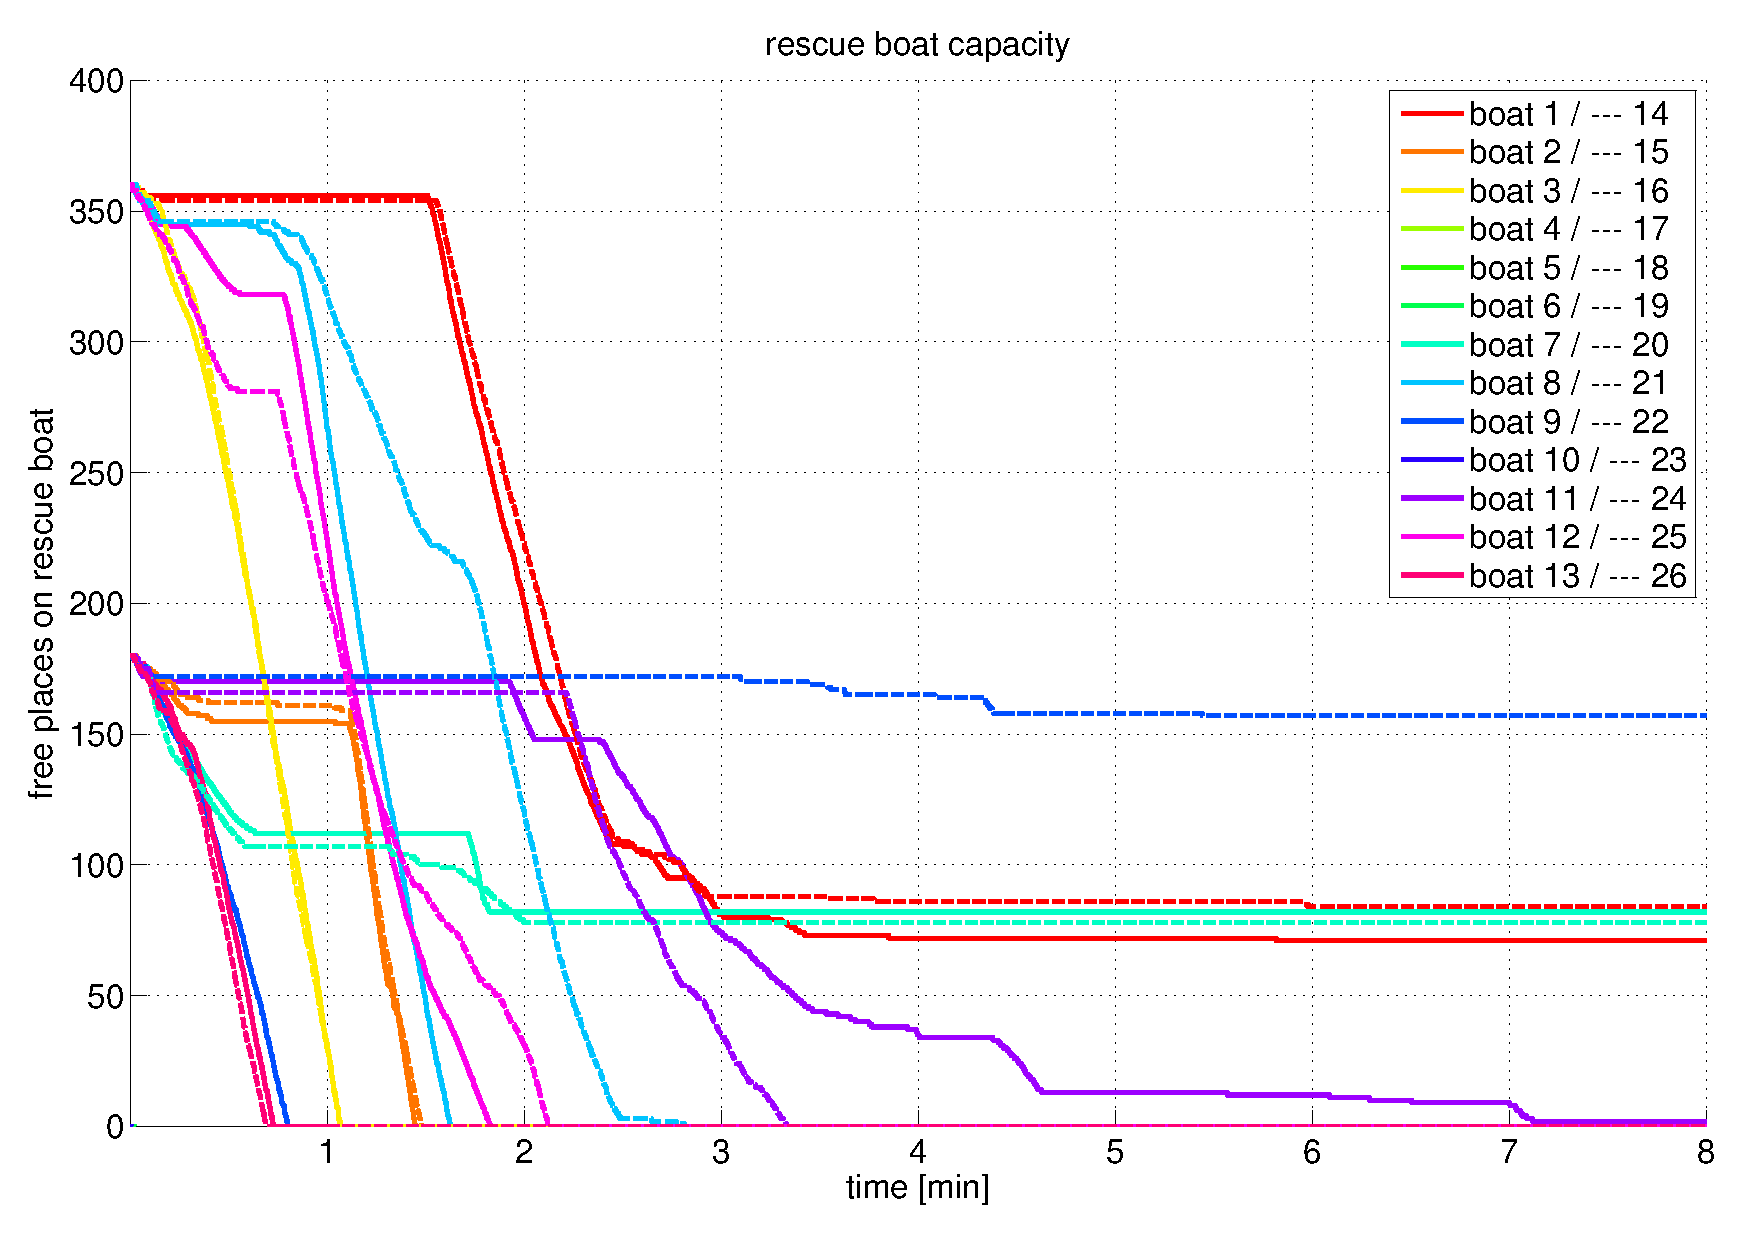
\includegraphics[width=\textwidth]{pics/vary_cap.pdf}
\caption{Varied boatsize simulation: Boat capacities during simulation}
\end{minipage}}
{\begin{minipage}[t]{7.4cm}
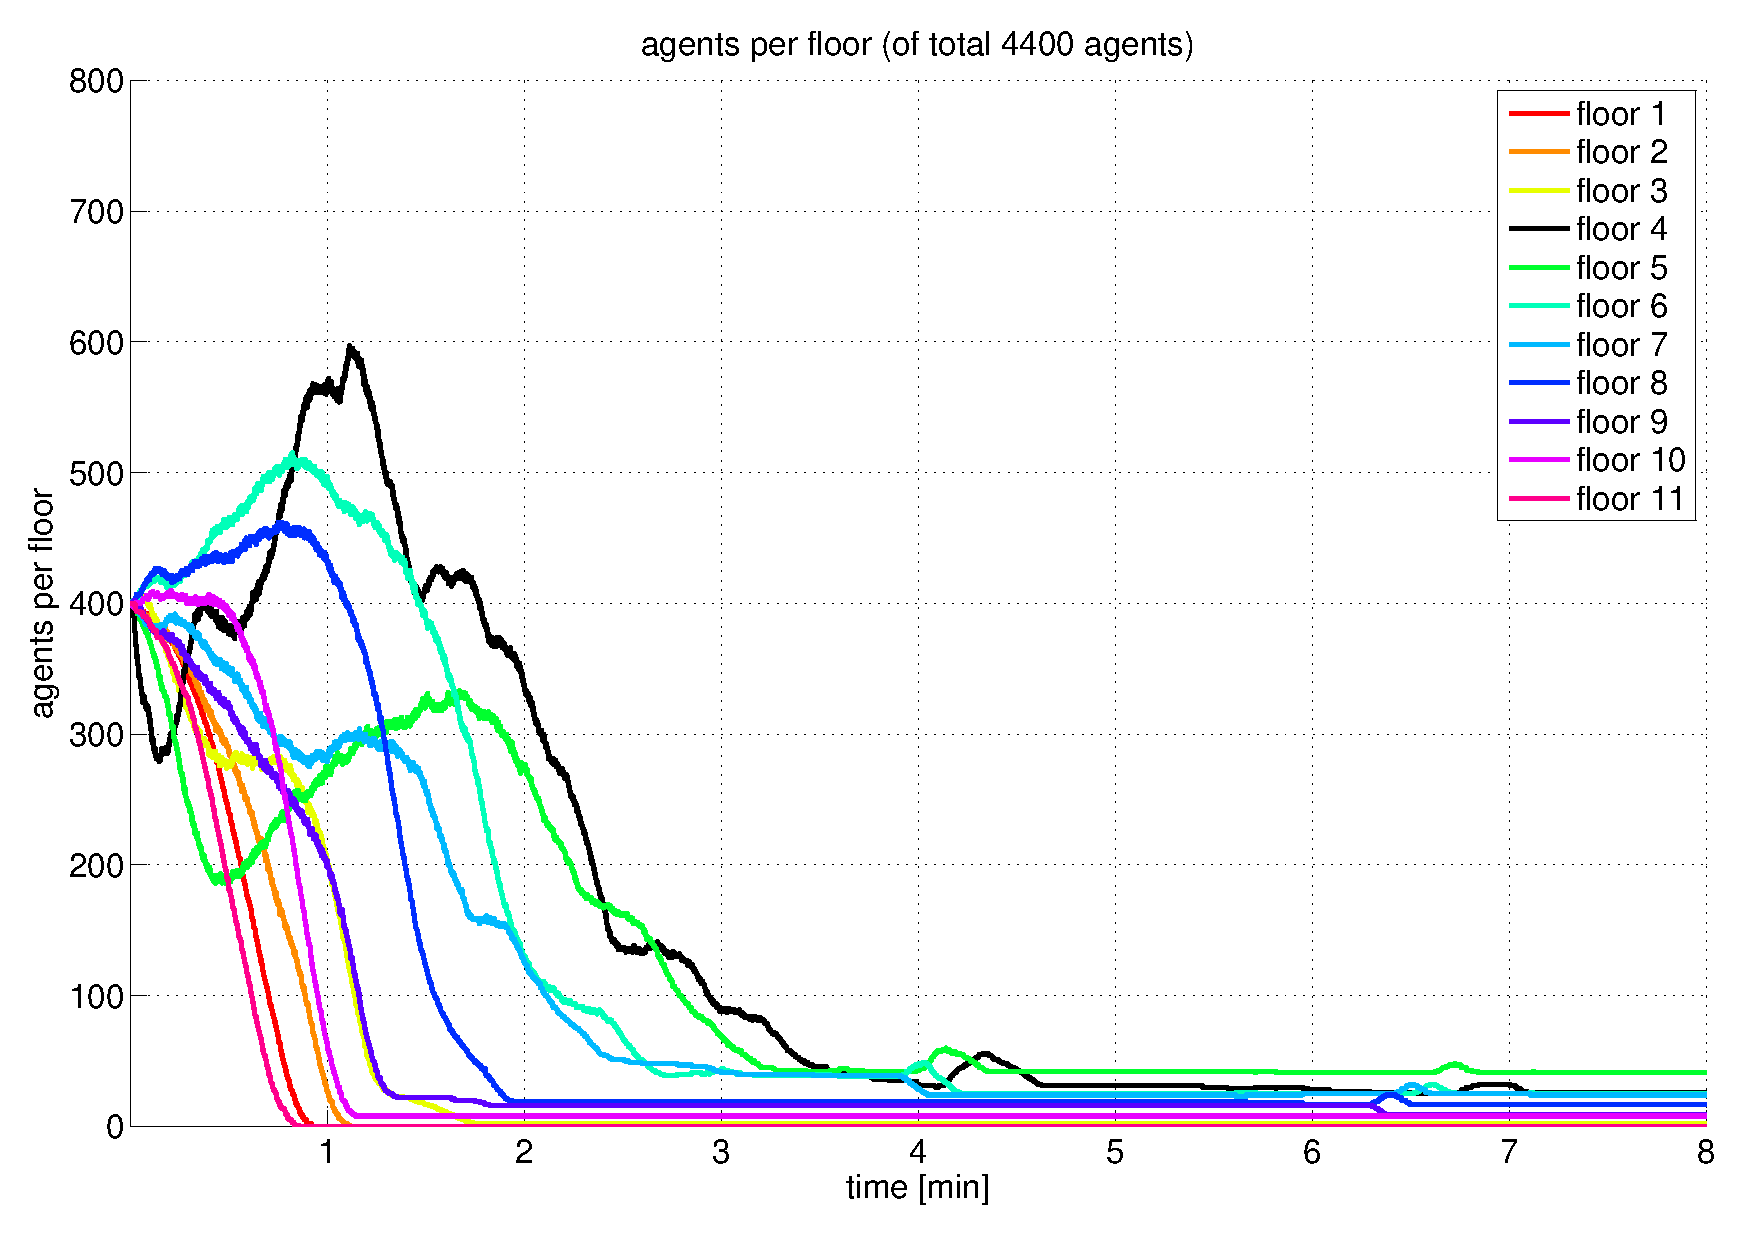
\includegraphics[width=\textwidth]{pics/vary_agents.pdf}
\caption{Varied boatsize simulation: Number of agents per floor}
\end{minipage}}
\end{figure}



\subsubsection{Crew command}

As already mentioned in the implementation part, we changed our code in order to simulate staff controlling the rescue situation. The results of that extention can be seen below. 


\begin{table}[H]
\centering
\begin{tabular}
{|>{\large}m{2cm} |>{\center}b{1.1cm} |>{\center}b{1.1cm}|>{}b{1.1cm}|>{}b{1.1cm}|} \hline \hline
percentage of agents & 10\% &  50\% & 90\% & 95\% \\ \hline
evacuation time & 20s &78s & 162s & 219s \\ \hline \hline
\end{tabular}
\caption{Crew command implementation: Needed time to evacuate a certain percentage of all agents.}
\end{table}


\begin{figure}[H]
\centering
{\begin{minipage}[t]{7.4cm}
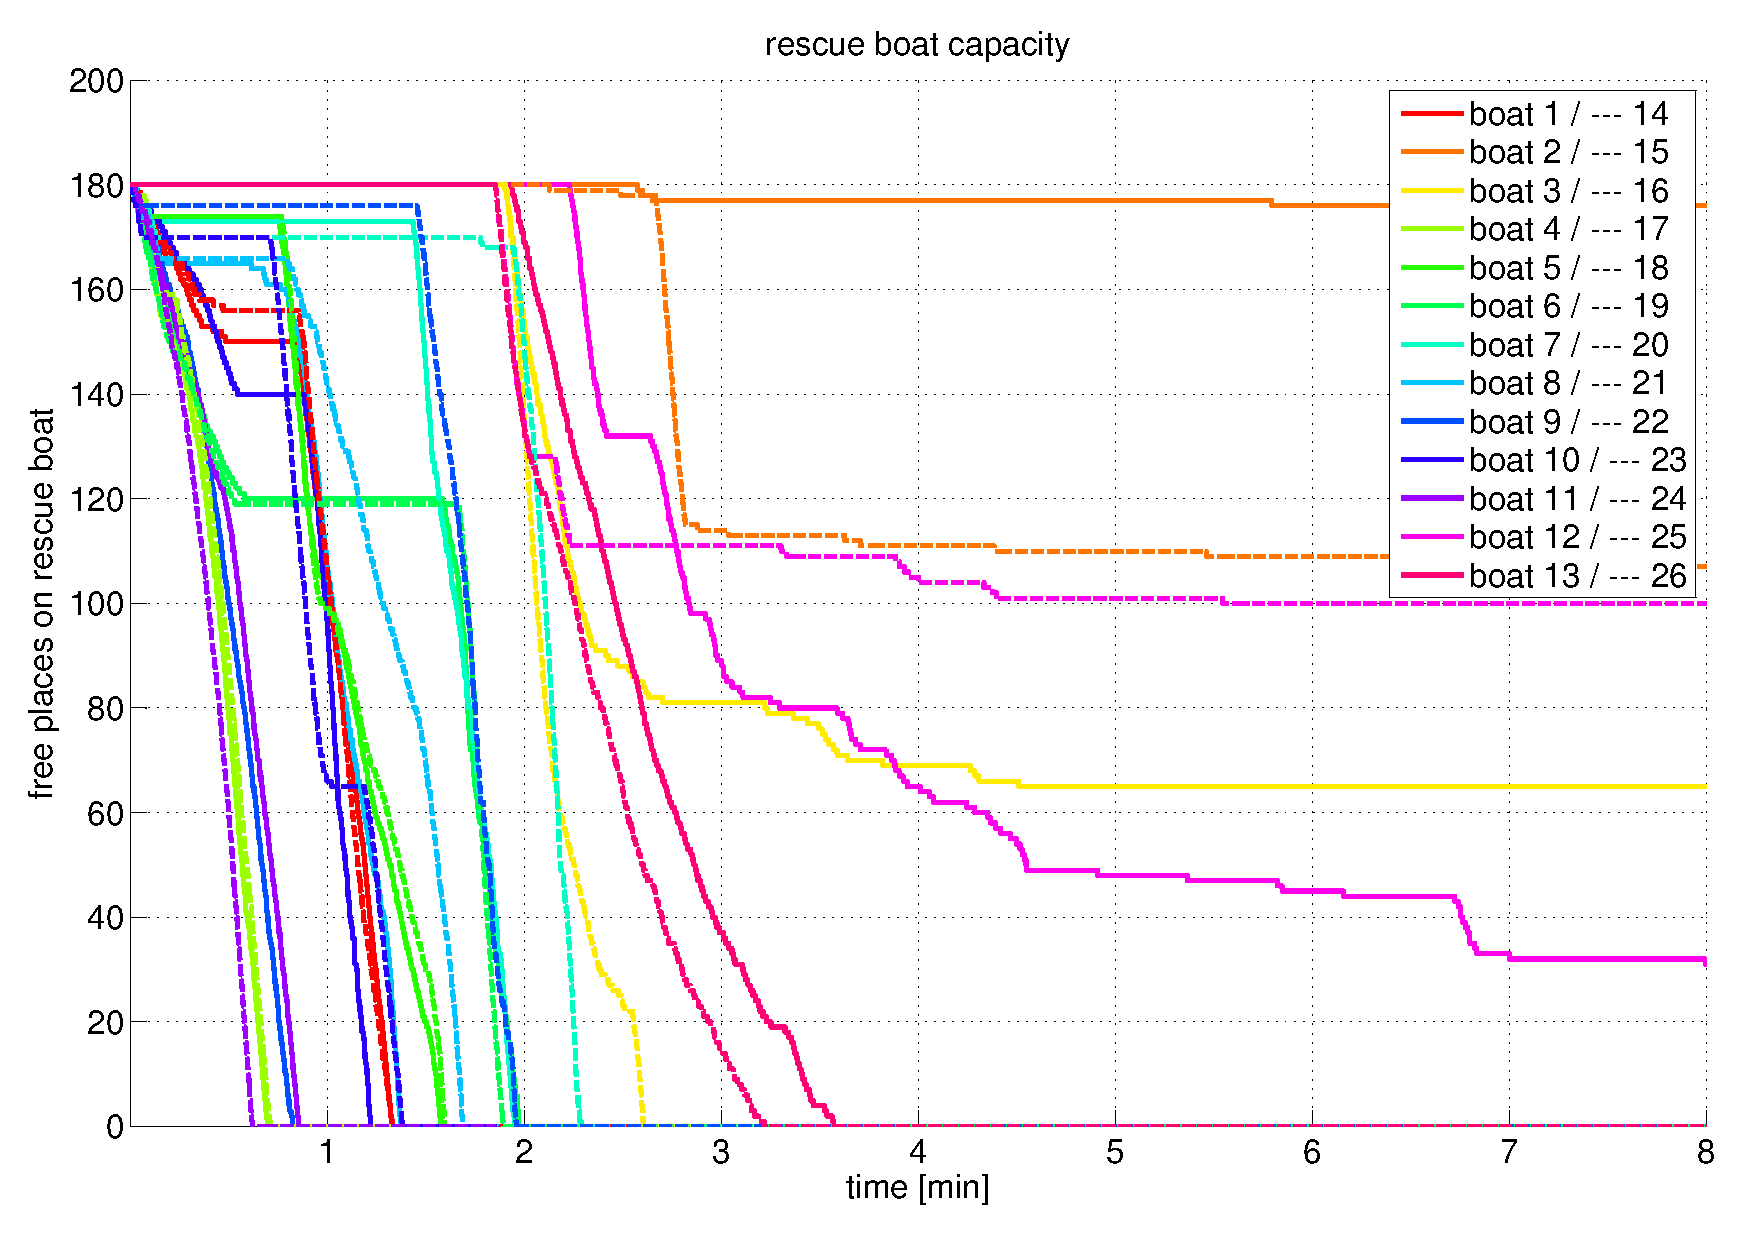
\includegraphics[width=\textwidth]{pics/crew_cap.pdf}
\caption{Crew command simulation: Boat capacities during simulation}
\end{minipage}}
{\begin{minipage}[t]{7.4cm}
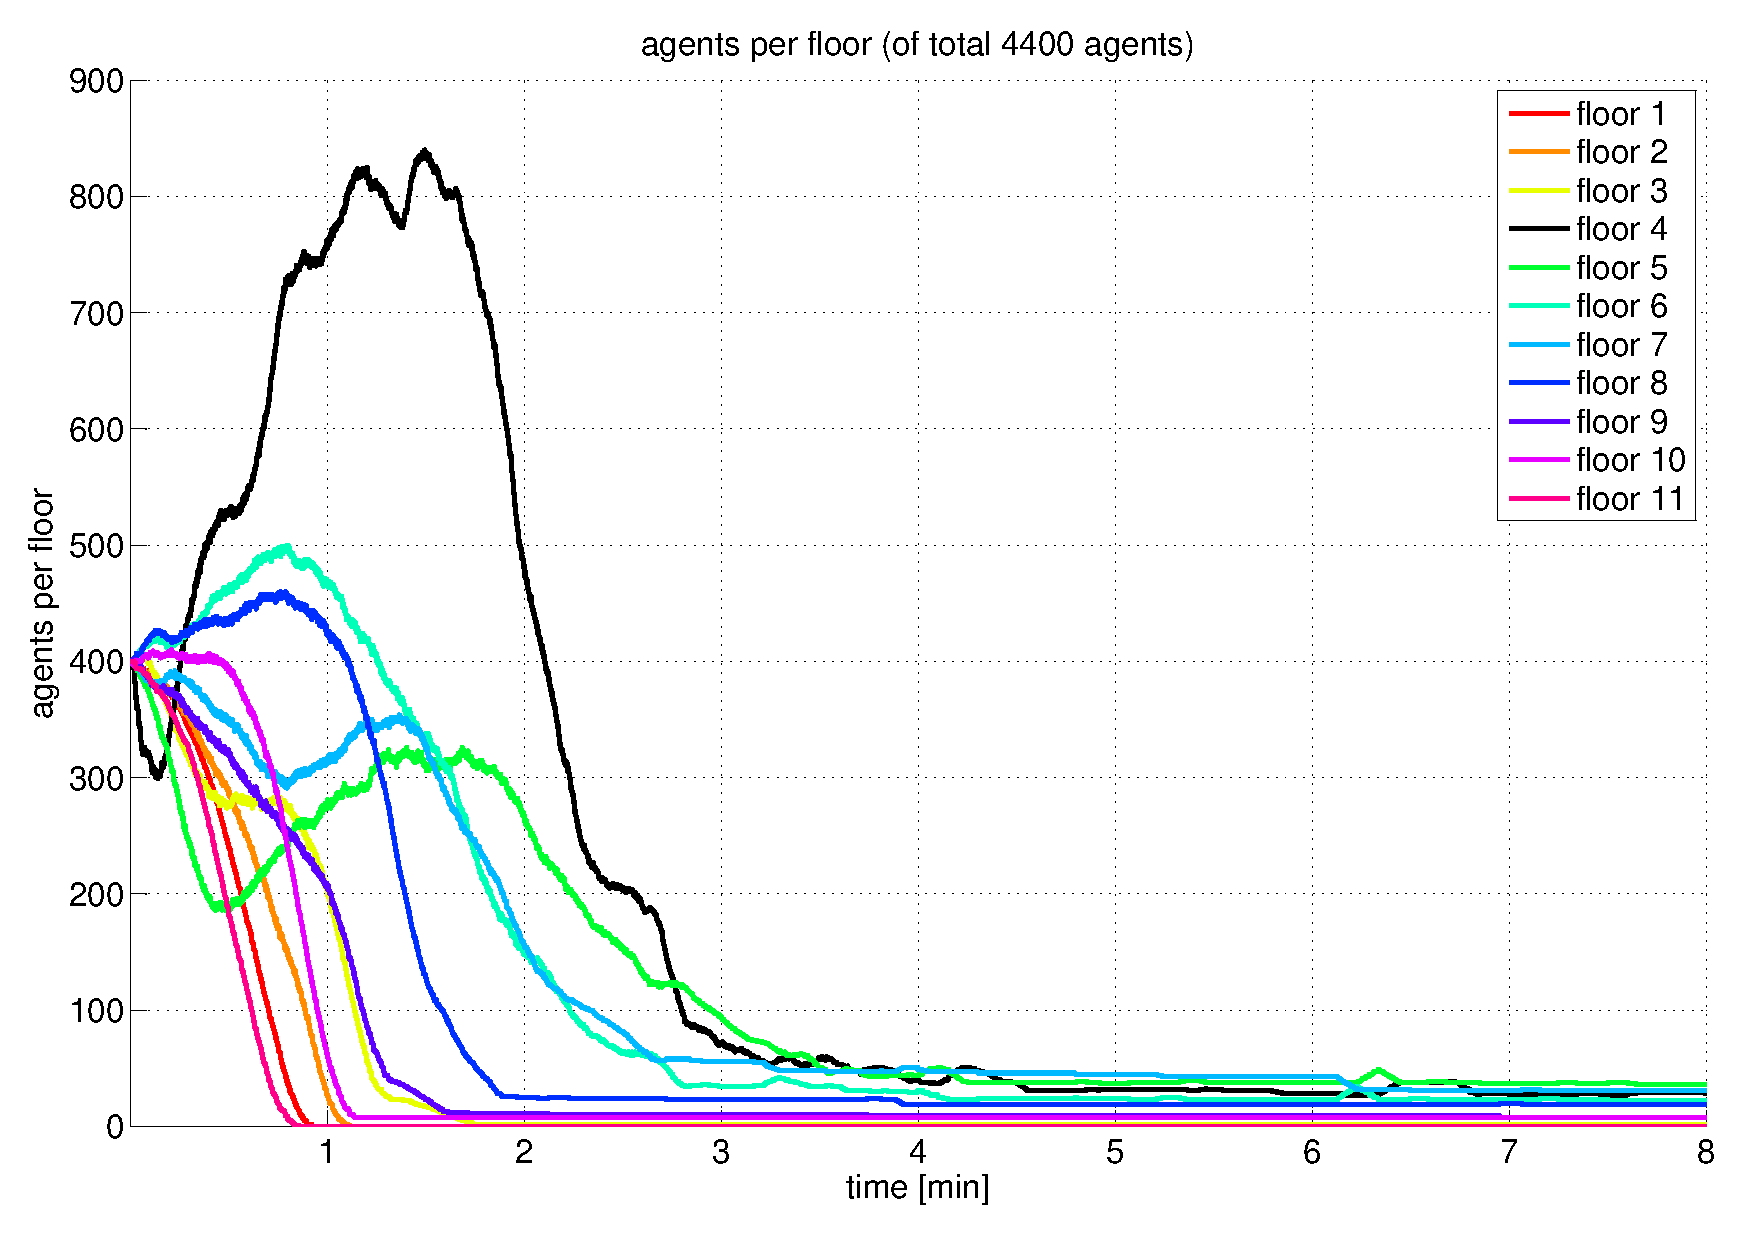
\includegraphics[width=\textwidth]{pics/crew_agents.pdf}
\caption{Crew command simulation: Number of agents per floor}
\end{minipage}}
\end{figure}




\subsection{Comparison}
\subsubsection{Standard - Modified room disposition}
The Analysis of the simulation results showed that there is a huge potential in saving evacuation time. By adding just one additional staircase we were able to reduce the overall evacuation time by 42 seconds. Further 50\% of all agents entered the exits approximately 2 seconds earlier compared to the stanard model. In contrast to that the rescueboat capacity utilisation remains basically the same.
\subsubsection{Standard - Modified rescueboat size}

As the results above show, there is no significant acceleration in the first part of the evacuation achieved by changing the distribution of the lifeboats .  
But, there is clearly a difference in the second half of the evacuation. The last 5\% of agents are evacuated 23 seconds faster what is a huge speed up.
This decrease in evacuation time is an effect of the reduced time the last agents need to leave the exit-deck.

\subsubsection{Standard - Crew command}
The results of the crew command extention are rather disappointing. On the one hand it was clear, that the first part of the simulation would become slower because the agents do not use the nearest boat. But on the other hand it was mentioned that the last part of the simulation has a significant speed up what is not the case. By looking at the video output the reason can be seen: The opening of the rescue boats near the stairs is useless at the point when only a few passengers are left because then they are already on the exit floor and walked towards the middle of the ship.\\
However, the idea has not to be thrown away. An implementation with a continuous opening of the next outer boat when the midmost ones are filled would eliminate our problem and a faster total evacuation time could be reached.

\subsection{General discussion}

During our project we revealed a lot of adjustments which could make cruise ships saver. Definitely we are aware of the simplicity of our model. Nevertheless we achieved to decrease the evacuation time with our improvements as shown above. Further we were able to attest that the staircases are the bottlenecks and it is possible to save time by adapting the ship geometry. Due to lack of time and simulation problems we unfortunately did not manage to find the optimal rescueboat size. However we proved that there is a capability to save further time by varying its size and position.


\section{Outlook}
During our work, we found a lot of possibilites to improve the model. The target of an ongoing project could be to make the model more realistic. There are a lot of possibilites to achieve this goal.
\newline
Some suggestions:
\begin{itemize}
\item To take into account that not all people automatically know where exactly the nearest exit is, the initialisation of the escape routes should be modified.
\item In our model the agents are evenly distributed over the floors and decks at the beginning of the simulation. This is however a very unrealistic scenario. In reality the agents will be uneavenly spread. The evacuation time would depend very much on the form of this distribution.
\item Different scenarios like night, dinner-time etc. that would change the distribution of the agents significantly could be compared.
\item In reality there are a lot of effects that could occur like fire, tilt of the ship, flooded areas, power failure, mass panic etc.
\end{itemize}
There are a lot of other interesting effects that could be looked at as well.
\\
Some ideas:
\begin{itemize}
\item In the ideal case, the evacuations on a ship are planned well. A good idea would be to define specific control points at which agents gahter first. From those points the agents would be led in small groups to the rescueboats by a crew member. It would be interesting to analyse the effect of such a efficient control.
\item The optimal combination of the different modifications we analyzed in this project could be found and therefore a minimal evacuation time.
\end{itemize}
For sure further interesting outcomes could be made by simply merging our results, means for example varying rescueboat size and geometries.
\section{References}

\begin{thebibliography}{9}
\bibitem{Helbling} Helbing, Dirk (1995): Social Force Model for Pedestrians Dynamics.
\bibitem{EscapePanic} Helbling, Dirk et al (2000): Simulating dynamical features of escape panic.
\bibitem{Building} Hardmeier,Jenal,Kueng,Thaler (2012): Modelling Situations of Evacuation in a Multi-level Building.
\bibitem{SOLAS} SOLAS (1974): International Convention for the Safety of Life at Sea. \url{http://www.imo.org/about/conventions/listofconventions/pages/international-convention-for-the-safety-of-life-at-sea-(solas),-1974.aspx}
\bibitem{ship} SHIP EVACUATION: \url{http://www.shipevacuation.com/}
\bibitem{shipdecks} CRUISE DECK PLANS PUBLIC SITE: \url{http://www.cruisedeckplans.com/DP/Main/decks.php?ship=Costa Serena}
\bibitem{EXODUS} University of Greenwich (2011):  maritimeEXODUS. \url{http://fseg.gre.ac.uk/fire/marine_evac_model.html}
\bibitem{concordia} Haverie of Costa Concordia (2012): \url{http://de.wikipedia.org/wiki/Costa_Concordia#Havarie_2012}
	
\end{thebibliography}
\section{Appendix}

\subsection{Code}

% define colors
\definecolor{commentcolor}{RGB}{89, 168, 89}
\definecolor{keywordcolor}{RGB}{68, 68, 255}
\definecolor{stringcolor}{RGB}{205, 139, 247}
\definecolor{numbercolor}{RGB}{128, 128, 128}
\definecolor{bgcolor}{RGB}{245, 248, 253}

% define listings style
\lstset{
  language=Matlab,
  basicstyle=\footnotesize\ttfamily,
  numbers=left,
  numberstyle=\tiny\color{numbercolor},
  stepnumber=2,
  numbersep=5pt,
  backgroundcolor=\color{bgcolor},
  showspaces=false,
  showstringspaces=false,
  showtabs=false,
  frame=lines,
  rulecolor=\color{black},
  tabsize=2,
  captionpos=b,
  breaklines=true,
  breakatwhitespace=true,
  title=\lstname,
  commentstyle=\color{commentcolor},
  keywordstyle=\color{keywordcolor},
  stringstyle=\color{stringcolor}
}

\subsubsection{\textit{standard} code}

\lstinputlisting[caption=addAgentRepulsiveForce.m]{../../code/addAgentRepulsiveForce.m}
\lstinputlisting[caption=addDesiredForce.m]{../../code/addDesiredForce.m}
\lstinputlisting[caption=addWallForce.m]{../../code/addWallForce.m}
\lstinputlisting[caption=applyForcesAndMove.m]{../../code/applyForcesAndMove.m}
\lstinputlisting[caption=checkForIntersection.m]{../../code/checkForIntersection.m}
\lstinputlisting[caption=compileC.m]{../../code/compileC.m}
\lstinputlisting[caption=initAgents.m]{../../code/initAgents.m}
\lstinputlisting[caption=initEscapeRoutes.m]{../../code/initEscapeRoutes.m}
\lstinputlisting[caption=initialize.m]{../../code/initialize.m}
\lstinputlisting[caption=initWallForces.m]{../../code/initWallForces.m}
\lstinputlisting[caption=loadConfig.m]{../../code/loadConfig.m}
\lstinputlisting[caption=plotAgentsPerFloor.m]{../../code/plotAgentsPerFloor.m}
\lstinputlisting[caption=plotExitedAgents.m]{../../code/plotExitedAgents.m}
\lstinputlisting[caption=plotFloor.m]{../../code/plotFloor.m}
\lstinputlisting[caption=plotFloor.m]{../../code/postprocessing.m}
\lstinputlisting[caption=simulate.m]{../../code/simulate.m}


%
%
%\subsubsection{\textit{control exit} code}
%
%\lstinputlisting[caption=addAgentRepulsiveForce.m]{../../code_control_exit/addAgentRepulsiveForce.m}
%\lstinputlisting[caption=addDesiredForce.m]{../../code_control_exit/addDesiredForce.m}
%\lstinputlisting[caption=addWallForce.m]{../../code_control_exit/addWallForce.m}
%\lstinputlisting[caption=applyForcesAndMove.m]{../../code_control_exit/applyForcesAndMove.m}
%\lstinputlisting[caption=checkForIntersection.m]{../../code_control_exit/checkForIntersection.m}
%\lstinputlisting[caption=compileC.m]{../../code_control_exit/compileC.m}
%\lstinputlisting[caption=initAgents.m]{../../code_control_exit/initAgents.m}
%\lstinputlisting[caption=initEscapeRoutes.m]{../../code_control_exit/initEscapeRoutes.m}
%\lstinputlisting[caption=initEscapeRoutes\_even.m]{../../code_control_exit/initEscapeRoutes_even.m}
%\lstinputlisting[caption=initEscapeRoutes\_odd.m]{../../code_control_exit/initEscapeRoutes_odd.m}
%\lstinputlisting[caption=initialize.m]{../../code_control_exit/initialize.m}
%\lstinputlisting[caption=initWallForces.m]{../../code_control_exit/initWallForces.m}
%\lstinputlisting[caption=loadConfig.m]{../../code_control_exit/loadConfig.m}
%\lstinputlisting[caption=plotAgentsPerFloor.m]{../../code_control_exit/plotAgentsPerFloor.m}
%\lstinputlisting[caption=plotExitedAgents.m]{../../code_control_exit/plotExitedAgents.m}
%\lstinputlisting[caption=plotFloor.m]{../../code_control_exit/plotFloor.m}
%\lstinputlisting[caption=plotFloor.m]{../../code_control_exit/postprocessing.m}
%\lstinputlisting[caption=simulate.m]{../../code_control_exit/simulate.m}


\subsubsection{\textit{C} code}

\lstinputlisting[language=C,caption=createRangeTree.c]{../../code/createRangeTree.c}
\lstinputlisting[language=C,caption=fastSweeping.c]{../../code/fastSweeping.c}
\lstinputlisting[language=C,caption=getNormalizedGradient.c]{../../code/getNormalizedGradient.c}
\lstinputlisting[language=C,caption=lerp2.c]{../../code/lerp2.c}
\lstinputlisting[language=C,caption=rangeQuery.c]{../../code/rangeQuery.c}
\lstinputlisting[language=C,caption=tree.h]{../../code/tree.h}
\lstinputlisting[language=C,caption=tree\_build.h]{../../code/tree_build.h}
\lstinputlisting[language=C,caption=tree\_build.c]{../../code/tree_build.c}
\lstinputlisting[language=C,caption=tree\_free.c]{../../code/tree_free.c}
\lstinputlisting[language=C,caption=tree\_query.h]{../../code/tree_query.h}
\lstinputlisting[language=C,caption=tree\_query.c]{../../code/tree_query.c}
\lstinputlisting[language=C,caption=tree\_types.h]{../../code/tree_types.h}


\subsubsection{\textit{crew command} code}

\lstinputlisting[caption=addAgentRepulsiveForce.m]{../../code_crew_command/addAgentRepulsiveForce.m}
\lstinputlisting[caption=addDesiredForce.m]{../../code_crew_command/addDesiredForce.m}
\lstinputlisting[caption=addWallForce.m]{../../code_crew_command/addWallForce.m}
\lstinputlisting[caption=applyForcesAndMove.m]{../../code_crew_command/applyForcesAndMove.m}
\lstinputlisting[caption=checkForIntersection.m]{../../code_crew_command/checkForIntersection.m}
\lstinputlisting[caption=compileC.m]{../../code_crew_command/compileC.m}
\lstinputlisting[caption=initAgents.m]{../../code_crew_command/initAgents.m}
\lstinputlisting[caption=initEscapeRoutes.m]{../../code_crew_command/initEscapeRoutes.m}
\lstinputlisting[caption=initialize.m]{../../code_crew_command/initialize.m}
\lstinputlisting[caption=initWallForces.m]{../../code_crew_command/initWallForces.m}
\lstinputlisting[caption=loadConfig.m]{../../code_crew_command/loadConfig.m}
\lstinputlisting[caption=plotAgentsPerFloor.m]{../../code_crew_command/plotAgentsPerFloor.m}
\lstinputlisting[caption=plotExitedAgents.m]{../../code_crew_command/plotExitedAgents.m}
\lstinputlisting[caption=plotFloor.m]{../../code_crew_command/plotFloor.m}
\lstinputlisting[caption=simulate.m]{../../code_crew_command/simulate.m}



\end{document}  

 
